\documentclass[12pt,a4paper,titlepage]{article}

% ============================================================
%  Packages généraux
% ============================================================
\usepackage[utf8]{inputenc}
\usepackage[T1]{fontenc}
\usepackage[french]{babel}
\usepackage{fontspec}
\setmainfont{Latin Modern Roman}
\usepackage{amsmath, amsfonts, amssymb}
\usepackage{graphicx}
\usepackage{hyperref}
\usepackage{geometry}
\usepackage{booktabs}
\usepackage{array}
\usepackage{longtable}
\usepackage{enumitem}
\usepackage{float}
\usepackage[table]{xcolor}
\usepackage{tabularx}
\usepackage{etoolbox}
\usepackage{titlesec}
\usepackage{abstract}
\usepackage{setspace}
\usepackage{caption}
\usepackage{adjustbox}
\usepackage{listings}
\usepackage{tikz}
\usetikzlibrary{arrows.meta, positioning}
\usepackage{pgfplots}
\pgfplotsset{compat=1.18}

% ============================================================
%  Style des tableaux
% ============================================================
% colortbl récent + array antérieur à 2024 (MiKTeX non à jour) : macro manquante
\makeatletter\providecommand\insert@pcolumn{\insert@column}\makeatother
\definecolor{tabhead}{RGB}{31,78,121}
\definecolor{tabstripe}{RGB}{242,246,250}
\definecolor{tabchoice}{RGB}{222,238,212}
\newcolumntype{L}{>{\raggedright\arraybackslash}X}
\newcolumntype{C}{>{\centering\arraybackslash}X}
\newcolumntype{F}[1]{>{\raggedright\arraybackslash\bfseries\leavevmode\color{tabhead}}p{#1}}
\newcommand{\hd}[1]{\textcolor{white}{\textbf{#1}}}
\newcommand{\choix}{\rowcolor{tabchoice}}
\setlength{\aboverulesep}{0pt}
\setlength{\belowrulesep}{0pt}
\setlength{\heavyrulewidth}{1pt}
% \small ici serait annulé par \@floatboxreset : on le place sur les tabulaires
\AtBeginEnvironment{tabularx}{\small}
\AtBeginEnvironment{tabular}{\small}
\AtBeginEnvironment{table}{%
  \renewcommand{\arraystretch}{1.45}%
  \arrayrulecolor{tabhead}%
  \rowcolors{2}{white}{tabstripe}%
}
\captionsetup{font=small, labelfont={bf,color=tabhead}, labelsep=period}
\captionsetup[table]{skip=6pt}

% ============================================================
%  Style des graphiques comparatifs
% ============================================================
\definecolor{cChoix}{RGB}{31,78,121}
\definecolor{cAltA}{RGB}{237,125,49}
\definecolor{cAltB}{RGB}{165,165,165}
\definecolor{cAltC}{RGB}{255,192,0}
\pgfplotsset{
  choix/.style={fill=cChoix, draw=cChoix!70!black, area legend},
  altA/.style={fill=cAltA, draw=cAltA!70!black, area legend},
  altB/.style={fill=cAltB, draw=cAltB!70!black, area legend},
  altC/.style={fill=cAltC, draw=cAltC!70!black, area legend},
  rapport/.style={
    axis lines*=left,
    axis line style={gray!70},
    ymajorgrids, grid style={dashed, gray!30},
    tick style={draw=none},
    tick label style={font=\small},
    label style={font=\small},
    legend cell align=left,
    legend style={draw=none, fill=none, font=\small, /tikz/every even column/.append style={column sep=10pt}},
  },
  comparatif/.style={
    rapport,
    ybar, bar width=10pt,
    width=0.93\textwidth, height=6.5cm,
    ymin=0, ymax=5.9, ytick={0,1,...,5},
    ylabel={Score qualitatif (0--5)},
    xtick=data,
    x tick label style={font=\small, align=center, text width=3cm},
    legend style={at={(0.5,1.02)}, anchor=south, legend columns=-1},
    nodes near coords, nodes near coords style={font=\scriptsize, color=black!70},
  },
}

% ============================================================
%  Géométrie de page
% ============================================================
\geometry{
  top=2.5cm, bottom=2.5cm,
  left=2.5cm, right=2.5cm
}
\onehalfspacing

\newtheorem{definition}{Définition}[section]

% ============================================================
%  Style des listings de code
% ============================================================
\lstset{
  basicstyle=\ttfamily\small,
  breaklines=true,
  frame=single,
  backgroundcolor=\color{gray!5},
  columns=fullflexible,
  keywordstyle=\color{blue!60!black}\bfseries,
  commentstyle=\color{green!40!black}\itshape,
  stringstyle=\color{orange!70!black},
  showstringspaces=false
}

\begin{document}

% ============================================================
%  PAGE DE TITRE
% ============================================================
\begin{titlepage}
    \centering

    \IfFileExists{INPT.png}{
        \begin{figure}[h]
            \raggedleft
            
\includegraphics[width=0.35\linewidth]{INPT.png}
        \end{figure}
    }{
        \begin{flushright}
            \fbox{\parbox{0.35\linewidth}{\centering\vspace{1.2cm}\textit{[Logo INPT]}\vspace{1.2cm}}}
        \end{flushright}
    }

    \vspace*{0.5cm}
    {\Large\bfseries Institut National des Postes et Télécommunications}\\[0.3cm]
    \vspace*{0.5cm}

    {\Huge\bfseries Semantic Digital Mapping}\\[0.3cm]
    {\Huge\bfseries via Vision-Assisted ISAC}\\[0.8cm]
    {\LARGE\bfseries Rapport de Projet de Fin d'Année}\\[0.4cm]
    {\large\itshape Positionnement, conception, mise en \oe uvre et résultats\\ d'un pipeline de cartographie sémantique par fusion ISAC-vision}\\[3cm]

    \begin{minipage}{0.8\textwidth}
        \centering
        \textbf{Auteur :}\\[0.2cm]
        LAZAAR EL MEHDI\\[0.5cm]
        EL KARFI SOUFIA\\[0.5cm]
        \textbf{Encadrement :}\\[0.2cm]
        CHAFNAJI HOUDA\\[0.5cm]
        \textbf{Contexte :}\\[0.2cm]
        Projet de Fin d'Année -- Réseaux 6G et IA Appliquée
    \end{minipage}

    \vfill

    {\large Année 2026}

\end{titlepage}

\newpage
\tableofcontents
\newpage

% ============================================================
\section{Introduction Générale}
% ============================================================

\subsection{Contexte : la mutation des réseaux post-6G}

À l'horizon des dix prochaines années, l'écosystème des télécommunications civiles et industrielles subira une mutation caractérisée par la transition d'applications centrées sur l'échange de données à des architectures d'immersion totale --- métavers persistant, sociétés holographiques interconnectées, systèmes industriels cyber-physiques. Ces applications se distinguent des services phares de la 5G/6G (\textit{eMBB}, \textit{URLLC}, \textit{ITS}) par leur nature multidimensionnelle : elles exigent la convergence immédiate des communications ultra-haut débit, du calcul distribué (\textit{Edge/Fog Computing}), de la détection environnementale active (\textit{Integrated Sensing and Communications}, ISAC) et de l'intelligence artificielle décentralisée.

Depuis la 2G, l'ingénierie des réseaux a suivi une trajectoire d'extrapolation incrémentale de l'équation de capacité de Shannon : ouverture spectrale (mmWave, sub-THz), densification spatiale (MIMO massif, surfaces intelligentes reconfigurables), réutilisation du spectre. Cette approche se heurte désormais à des limites physiques dures --- couplage d'antennes aux échelles sub-longueur d'onde, sensibilité extrême aux blocages en bande THz, complexité asymptotique du précodage en champ proche --- qui dépassent les capacités thermiques et énergétiques des stations de base actuelles.

Pour répondre à ces limites, la première phase de la 6G a introduit le réseau nativement IA (\textit{AI-native}), fondé sur le déploiement de réseaux de neurones profonds à travers la pile protocolaire. Cette IA statistique de première génération présente toutefois des failles structurelles : absence de causalité (les corrélations apprises s'effondrent hors distribution), dilemme stabilité-plasticité (\textit{catastrophic forgetting} vs rigidité), et coût prohibitif du réentraînement périodique à la périphérie du réseau. C'est cette impasse qui motive le saut vers des \textbf{systèmes sans fil natifs AGI} (\textit{Artificial General Intelligence-Native}), capables de raisonner sur leurs propres contraintes physiques plutôt que d'ajuster des courbes de probabilités --- cadre détaillé en \S\ref{subsec:telecom_brain}.

\subsection{Problématique}

Deux architectures récentes formalisent cette transition sous des angles complémentaires : le \textit{Telecom Brain} AGI-natif de Saad~\textit{et al.}~\cite{saad2025}, qui propose un cadre cognitif complet (perception, modèle du monde causal, planification) sans préciser comment les représentations sémantiques sont construites à partir des signaux physiques bruts ; et l'architecture Semantic-Aware Vision-Assisted ISAC (SA-VA-ISAC), qui fusionne concrètement ISAC et vision pour l'allocation de ressources, mais se limite à une exploitation tactique locale, sans mémoire long terme ni raisonnement contrefactuel. \textbf{Aucune des deux ne spécifie comment une carte sémantique 3D temps réel de l'environnement radio est effectivement construite, maintenue et compressée} --- le pont entre couche physique et cognition de haut niveau reste abstrait.

\subsection{Objectifs et contributions du projet}

Le projet \textbf{SDM-VA-ISAC} (\textit{Semantic Digital Mapping via Vision-Assisted ISAC}) répond à cette lacune en opérationnalisant ce pont : un pipeline de perception qui fusionne acquisition ISAC (radar) et acquisition vision (caméra RGB) pour construire, incrémentalement, une carte sémantique 3D compressée par encodage hyperdimensionnel, simulée de bout en bout avec NVIDIA Sionna sur une scène urbaine réelle. Ce rapport documente :
\begin{enumerate}[leftmargin=1.5em]
    \item la revue de littérature complète ayant motivé et positionné le projet (\S\ref{sec:etat_art}) ;
    \item l'architecture globale proposée pour répondre à la problématique identifiée (\S\ref{sec:architecture_proposee}) ;
    \item les choix technologiques structurants, justifiés par comparaison explicite et visuelle avec leurs alternatives (\S\ref{sec:choix_tech}) ;
    \item la méthodologie effectivement suivie pour construire le pipeline de perception et de cartographie (\S\ref{sec:methodologie}) ;
    \item les résultats numériques obtenus et validés à chaque étape (\S\ref{sec:resultats}) ;
    \item les limitations rencontrées et le périmètre retenu, documentés honnêtement plutôt que masqués (\S\ref{sec:limitations}).
\end{enumerate}

\subsection{Plan du rapport}

La section~\ref{sec:etat_art} couvre l'ensemble de la revue de littérature : les architectures cognitives fondatrices (Telecom Brain, SA-VA-ISAC), leur convergence et la lacune scientifique identifiée, ainsi que les corpus techniques mobilisés par l'implémentation (ray tracing différentiable, détection temps réel, fusion multi-capteurs, cartographie sémantique, calcul hyperdimensionnel). La section~\ref{sec:architecture_proposee} présente l'architecture globale proposée pour SDM-VA-ISAC. La section~\ref{sec:choix_tech} détaille et justifie, tableaux et graphiques à l'appui, les choix technologiques. La section~\ref{sec:methodologie} décrit la méthodologie suivie, avec extraits de code. La section~\ref{sec:resultats} rapporte les résultats obtenus. La section~\ref{sec:limitations} synthétise le périmètre retenu. La section~\ref{sec:conclusion} conclut.

% ============================================================
\section{État de l'Art}
\label{sec:etat_art}
% ============================================================

\subsection{Systèmes sans fil nativement AGI : le \textit{Telecom Brain}}
\label{subsec:telecom_brain}

\subsubsection{La philosophie du \textit{common sense} cybernétique}

L'Intelligence Artificielle Générale appliquée aux télécommunications se caractérise par l'intégration d'un noyau de \textit{common sense} (bon sens), formalisé à travers quatre piliers~\cite{saad2025} :

\begin{itemize}[leftmargin=1.5em]
    \item \textbf{Généralisabilité horizontale} : transfert de l'expertise opérationnelle d'un agent entre domaines statistiquement disjoints ($\mathcal{D}_S \to \mathcal{D}_T$, $P(X_S) \neq P(X_T)$), sans phase de calibration empirique additionnelle, par exploitation d'invariants structurels.
    \item \textbf{Physique intuitive} : le réseau interprète les coefficients de canal (CSI) non comme de simples tenseurs, mais à la lumière des lois physiques sous-jacentes (optique géométrique, diffraction), réduisant l'espace de recherche des solutions d'optimisation.
    \item \textbf{Raisonnement analogique} : établissement d'isomorphismes relationnels entre un problème inédit et des structures causales déjà rencontrées, permettant une remédiation sans phase d'essais-erreurs destructrice de QoS.
    \item \textbf{Complétion de l'information} (\textit{filling in the blanks}) : reconstruction de l'état complet du champ électromagnétique à partir d'observations parcellaires et bruitées, par déduction causale plutôt que par acquisition exhaustive.
\end{itemize}

\subsubsection{Modèle du monde causal hyperdimensionnel}

Le \textit{Telecom Brain} formalise son modèle du monde par l'union de \textbf{Modèles Causaux Structurels} (SCM) et du \textbf{Calcul Hyperdimensionnel} (HD) :

\begin{definition}[Espace vectoriel causal HD]
L'espace du modèle du monde est un espace vectoriel hyperdimensionnel $\mathcal{V}_{HD} = \mathbb{R}^D$ avec $D \geq 10\,000$. Chaque entité $E$ est projetée en un vecteur pseudo-aléatoire dense $\mathbf{h}_E \in \mathcal{V}_{HD}$ satisfaisant $\langle \mathbf{h}_A, \mathbf{h}_B \rangle \approx 0$ pour deux entités indépendantes $A \neq B$.
\end{definition}

Trois opérateurs manipulent ces vecteurs : l'\textbf{addition} ($\mathbf{h}_{A+B} = \mathbf{h}_A + \mathbf{h}_B$, superposition sémantique), la \textbf{multiplication élément par élément} ($\odot$, liaison de concepts, ex. $\mathbf{h}_{concept} = \mathbf{h}_{freq} \odot \mathbf{h}_{position}$) et la \textbf{permutation} ($\Pi$, encodage de structures séquentielles). Un modèle causal structurel définit, pour chaque variable endogène $Y_i$, ses parents causaux $Pa(Y_i)$ et exogènes $U_i$ :
\begin{equation}
    Y_i = f_i(Pa(Y_i), U_i)
    \label{eq:scm}
\end{equation}
Ces équations, résolues algébriquement via les opérateurs HD, permettent l'évaluation instantanée d'interventions contrefactuelles ($P(QoS \mid \mathrm{do}(Puissance = P_{max}))$), l'isomorphisme entre l'espace physique du réseau et l'espace HD étant garanti par un foncteur préservant la structure $\mathcal{F} : \mathcal{C} \to \mathcal{H}$ (théorie des catégories).

\subsubsection{Planification et cas d'usage}

La planification se répartit entre une branche \textit{intent-driven} (gouvernance de haut niveau, fondée sur une adaptation de la théorie de l'information intégrée, indice $\Phi$) et une branche \textit{objective-driven} (décomposition hiérarchique descendante d'un macro-objectif en actions PHY/MAC/réseau à l'échelle de la milliseconde). Les cas d'usage phares incluent les \textbf{jumeaux numériques augmentés} (simulation contrefactuelle proactive avant l'action physique réelle), les \textbf{avatars cognitifs} (raisonnement abductif comblant les latences de transport pour le suivi oculaire/gestuel) et la \textbf{téléportation holographique} par \textit{Theory of Mind} (allocation de résolution guidée par l'attention visuelle du récepteur, réduction du débit d'un facteur $>100$).

\subsubsection{Insuffisance des LLM et impératif d'une IA ancrée dans la physique}

Le cadre de Saad~\textit{et al.} démontre que les grands modèles de langage (LLM) sont structurellement inadaptés à l'orchestration bas niveau des réseaux : ils opèrent sur des distributions statistiques de tokens sans ancrage sémantique dans la réalité physique (aucune compréhension d'une équation d'onde ou d'un bruit thermique), et leurs hallucinations comme leur latence les disqualifient des fonctions de contrôle temps réel. La recommandation stratégique est le développement d'une \textbf{IA ancrée dans la physique}, née de la fusion de la théorie de l'information sémantique, de la causalité de Pearl~\cite{pearl2009} et des lois de l'électromagnétisme. Le tableau~\ref{tab:agi_transition} synthétise cette transition.

\begin{table}[H]
    \centering
    \caption{Transition des réseaux 6G IA-natifs vers les réseaux post-6G AGI-natifs.}
    \label{tab:agi_transition}
    \begin{tabularx}{\textwidth}{F{3.4cm}LL}
        \toprule
        \rowcolor{tabhead}
        \hd{Caractéristique} & \hd{Réseaux 6G IA-Natifs} & \hd{Réseaux Post-6G AGI-Natifs} \\
        \midrule
        Paradigme fondamental & Statistique, corrélationnel, boîte noire & Causal, cognitif, explicable \\
        Abstraction mathématique & Réseaux de neurones profonds, descente de gradient & Théorie des catégories, algèbre hyperdimensionnelle, SCM \\
        Gestion de l'environnement & Réapprentissage permanent, adaptation passive & Physique intuitive, simulations contrefactuelles proactives \\
        Comportement face à l'inconnu & Effondrement des performances (\textit{catastrophic forgetting}) & Généralisabilité horizontale par raisonnement analogique \\
        \bottomrule
    \end{tabularx}
\end{table}

\subsection{Architecture Semantic-Aware Vision-Assisted ISAC (SA-VA-ISAC)}
\label{subsec:sa_va_isac}

\subsubsection{Motivation et composants}

L'explosion du trafic et la prolifération de services à très faible latence imposent deux contraintes : la congestion du c\oe ur de réseau par la transmission de données brutes issues de capteurs (caméras RGB-D, LiDAR, radar), et le besoin d'une perception environnementale continue pour adapter dynamiquement le \textit{beamforming}. L'architecture \textbf{SA-VA-ISAC} fusionne trois paradigmes --- ISAC, vision par ordinateur, communication sémantique --- pour maximiser l'efficacité énergétique (EE) et l'efficacité énergétique de confidentialité (SEE), tout en réduisant la charge backhaul.

Chaque \textbf{station de base VA-ISAC} embarque un réseau d'antennes multi-faisceau et un capteur RGB-D générant des nuages de points 3D en temps réel, assurant simultanément détection ISAC (position/vitesse des UE et obstacles) et transmission de données. Des \textbf{serveurs MEC} co-localisés hébergent l'agrégation d'informations multi-BS et les modèles de \textit{deep learning} pour l'allocation de ressources.

\subsubsection{Communication sémantique et codage source-canal conjoint}

La communication sémantique transmet le \textit{sens} de l'information plutôt que chaque bit. L'encodeur sémantique $f_{\boldsymbol{\theta}}$ produit une représentation latente $\mathbf{z} = f_{\boldsymbol{\theta}}(\mathbf{s})$, $\mathbf{z} \in \mathbb{R}^d$, $d \ll |\mathbf{s}|$, que le décodeur $g_{\boldsymbol{\phi}}$ reconstruit sous contrainte de distorsion sémantique maximale $\epsilon_{\mathrm{sem}}$ :
\begin{equation}
    \hat{\mathbf{s}} = g_{\boldsymbol{\phi}}(\tilde{\mathbf{z}}), \quad \text{s.c. } \mathcal{L}_{\mathrm{sem}}(\mathbf{s}, \hat{\mathbf{s}}) \leq \epsilon_{\mathrm{sem}}
    \label{eq:semantic_decoder}
\end{equation}
Le ratio de compression $\rho = d/|\mathbf{s}|$ peut atteindre $10^{-2}$, réduisant le trafic backhaul de plusieurs ordres de grandeur.

\subsubsection{Allocation de ressources par apprentissage profond}

L'objectif est la maximisation de l'efficacité énergétique $\mathrm{EE} = B \cdot R_{\mathrm{sum}} / P_{\mathrm{tot}}$, ou en présence d'écoutes passives $\mathcal{E}$, de l'efficacité énergétique de confidentialité $\mathrm{SEE} = B \sum_k R_k^{\mathrm{sec}} / P_{\mathrm{tot}}$, où $R_k^{\mathrm{sec}} = [\log_2(1+\mathrm{SINR}_k) - \max_{e\in\mathcal{E}} \log_2(1+\mathrm{SINR}_{k,e})]^+$. Ces problèmes non convexes et NP-difficiles sont résolus soit par un \textbf{DNN supervisé} (apprentissage hors ligne d'une correspondance $\boldsymbol{\xi}_t \to \{\mathbf{w}_k^*\}$, inférence en $\mathcal{O}(1)$ propagation avant), soit par \textbf{apprentissage par renforcement profond} (DRL, agent TD3/SAC sur un MDP dont l'état intègre le vecteur enrichi :
\begin{equation}
    \boldsymbol{\xi}_t = \left[ \mathrm{vec}(\mathbf{H}_t),\; \boldsymbol{\psi}_t^{\mathrm{ISAC}},\; \boldsymbol{\delta}_t^{\mathrm{CV}} \right]
    \label{eq:state_vector}
\end{equation}
où $\mathbf{H}_t$ est la matrice de canal, $\boldsymbol{\psi}_t^{\mathrm{ISAC}}$ les mesures radar et $\boldsymbol{\delta}_t^{\mathrm{CV}}$ la carte sémantique compressée issue de la vision.

Le tableau~\ref{tab:sa_va_isac_perf} résume les résultats publiés : un gain d'efficacité spectrale de 15--25\,\% par rapport au MIMO classique sans perception environnementale, et une réduction du temps de décision d'un facteur 100--400$\times$ par rapport aux méthodes itératives classiques (BSUM, SCA).

\begin{table}[H]
    \centering
    \caption{Performances publiées de SA-VA-ISAC vs. approches de référence~\cite{isac_survey,drl_beamforming}.}
    \label{tab:sa_va_isac_perf}
    \begin{tabularx}{\textwidth}{F{4.2cm}CCC}
        \toprule
        \rowcolor{tabhead}
        \hd{Métrique} & \hd{BSUM/SCA (réf.)} & \hd{DNN supervisé} & \hd{DRL (SA-VA-ISAC)} \\
        \midrule
        Efficacité spectrale & Haute (optimale) & $\approx 95\,\%$ de l'optimal & $\approx 97\,\%$ de l'optimal \\
        Temps de calcul (ms/itération) & 500--2000 & 2--5 & 3--8 \\
        Passage à l'échelle ($N_t$ grand) & Très faible & Modéré & Élevé \\
        Réduction trafic backhaul & Aucune & Partielle (JSCC) & Forte (JSCC + ISAC) \\
        \bottomrule
    \end{tabularx}
\end{table}

\subsection{Convergence des deux paradigmes et lacune scientifique identifiée}
\label{subsec:convergence}

\subsubsection{Points de convergence}

Bien que formulés dans des cadres distincts, les deux architectures convergent sur trois points : (i) la \textbf{primauté de la perception multimodale} --- fusion contrastive/CRL d'un côté, fusion RGB-D via ISAC de l'autre, vers une conscience situationnelle combinant informations spectrales, spatiales et sémantiques ; (ii) le \textbf{dépassement de la corrélation par la causalité} --- physique intuitive d'un côté, prédiction proactive du canal de l'autre ; (iii) la \textbf{compression sémantique} comme réponse à la saturation du backhaul --- \textit{Theory of Mind} et JSCC visant tous deux un ratio de compression $>100\times$ par modélisation des besoins informationnels réels du destinataire.

\begin{table}[H]
    \centering
    \caption{Matrice de complémentarité entre les deux architectures fondatrices.}
    \label{tab:complementarity}
    \begin{tabularx}{\textwidth}{F{3cm}LL}
        \toprule
        \rowcolor{tabhead}
        \hd{Dimension} & \hd{Apport AGI-Native (Saad~\textit{et al.})} & \hd{Apport SA-VA-ISAC} \\
        \midrule
        Abstraction & Théorie des catégories, calcul HD, SCM formel & Deep learning, optimisation EE/SEE \\
        Généralisation & Trans-domaines (raisonnement analogique) & Intra-domaine (DRL adaptatif en ligne) \\
        Planification & Hiérarchique intentionnelle (IIT) & Réactive (MDP, fonction de récompense) \\
        Passage à l'échelle & Abstraction catégorique préservant la structure & MEC local, apprentissage fédéré \\
        \bottomrule
    \end{tabularx}
\end{table}

\subsubsection{Verrous technologiques de la convergence}

Quatre verrous freinent la fusion effective des deux paradigmes : la \textbf{complexité de l'intégration mathématique} entre représentations HD bipolaires ($D\sim10^4$) et représentations continues apprises ($d\sim10^2$--$10^3$) ; la \textbf{latence de la boucle cognitive}, l'insertion d'un raisonnement causal supplémentaire (SCM, simulations contrefactuelles) risquant de dégrader la latence au-delà des seuils URLLC ($<1$~ms) ; la \textbf{cohérence des représentations distribuées} entre centaines de n\oe uds MEC maintenant chacun une vue locale partielle de l'espace HD global ; et l'\textbf{apprentissage des modèles causaux} eux-mêmes, la découverte causale à grande échelle (PC, FCI, LiNGAM) peinant à passer à l'échelle d'un réseau cellulaire complet sans contraintes physiques a priori.

\subsubsection{Lacune scientifique et contribution proposée}

Ni le \textit{Telecom Brain} ni SA-VA-ISAC ne spécifient \textbf{comment} une carte sémantique temps réel de l'environnement radio est concrètement construite à partir des signaux physiques bruts : SA-VA-ISAC se limite à une exploitation tactique locale (optimisation EE/SEE), sans mémorisation long terme ni raisonnement contrefactuel ; le \textit{Telecom Brain} propose un cadre cognitif complet mais ne spécifie pas la construction initiale des représentations sémantiques --- le pont entre couche PHY et \textit{World Model} reste abstrait. C'est cette lacune que \textbf{SDM-VA-ISAC} comble, en opérationnalisant la construction incrémentale d'une carte sémantique 3D par fusion ISAC + vision, servant de couche d'abstraction entre signaux physiques et modèle du monde causal --- architecture détaillée en \S\ref{sec:architecture_proposee}.

\subsection{Simulation de couche physique par ray tracing différentiable}
\label{subsec:art_rt}

La simulation de la propagation radio par lancer de rayons (\textit{ray tracing}) est une alternative aux modèles de canal statistiques (Rayleigh, Rician, 3GPP TR~38.901) lorsqu'une cohérence géométrique exacte entre la scène 3D et le canal radio est requise --- condition nécessaire pour fusionner ISAC et vision, puisque les deux modalités doivent partager le même repère spatial. NVIDIA Sionna RT~\cite{sionna_rt_2} introduit la différentiabilité du lancer de rayons par rapport aux paramètres de la scène (position, orientation, matériaux), ouvrant la voie à l'apprentissage de bout en bout --- une capacité absente des outils plus anciens tels que Wireless InSite (Remcom)~\cite{remcom_wi} ou le \textit{5G Toolbox} de MATLAB, qui reposent sur des moteurs propriétaires non différentiables et non scriptables pour la génération répétée de rendus annotés.

\subsection{Détection et segmentation d'objets en temps réel}
\label{subsec:art_detection}

La famille YOLO (\textit{You Only Look Once}) formule la détection d'objets comme un problème de régression unique plutôt que comme une cascade de propositions de régions (R-CNN, Faster R-CNN), ce qui la rend adaptée aux contraintes temps réel. YOLOv8~\cite{ultralytics_yolov8} ajoute une tête de segmentation d'instances (\textit{YOLOv8-seg}). SegFormer~\cite{segformer} propose une alternative fondée sur les Transformers, avec un décodeur MLP léger, offrant une meilleure qualité de segmentation dense au prix d'un coût de calcul supérieur.

Un problème récurrent lorsqu'un détecteur pré-entraîné sur des données réelles (COCO) est appliqué à des rendus synthétiques est l'\textit{écart de domaine sim-vers-réel}. La littérature propose la \textit{randomisation de domaine}~\cite{domain_randomization} (variation aléatoire de l'apparence synthétique) et le \textit{fine-tuning direct sur le domaine cible} (ré-entraînement sur des données annotées automatiquement dans le style du rendu de production) --- cette seconde famille est mobilisée dans ce projet (\S\ref{subsec:choix_vision_strategie}).

\subsection{Suivi multi-cibles et association temporelle}
\label{subsec:art_tracking}

Lorsqu'une séquence dynamique multi-frame est traitée, la littérature classique de fusion de capteurs distingue l'\textit{association instantanée} (associer, à un instant $t$, les mesures radar aux détections vision) du \textit{suivi temporel} (\textit{tracking}), qui maintient l'identité d'une cible à travers les frames malgré le bruit de mesure et les occultations transitoires. Les filtres de Kalman étendus/\textit{unscented} couplés à des méthodes d'association de type \textit{Multiple Hypothesis Tracking} ou \textit{Joint Probabilistic Data Association}~\cite{bar_shalom_tracking} sont la référence historique de ce second problème.

\subsection{Fusion radar-caméra et association de données}
\label{subsec:art_fusion}

L'association de détections issues de capteurs hétérogènes (nuage de points radar ISAC et masques de segmentation vision) est un problème classique de \textit{data association}. Les structures de type \textbf{arbre k-d} (\textit{k-d tree})~\cite{bentley_kdtree} permettent une recherche du plus proche voisin en $\mathcal{O}(\log n)$ et constituent la solution la plus simple pour l'association spatiale lorsque le nombre de cibles reste modéré. Des méthodes plus sophistiquées existent --- l'algorithme hongrois pour une association optimale globale, ou le JPDA en présence d'incertitude de mesure élevée --- au prix d'une complexité supérieure.

\subsection{Cartographie par grille d'occupation et cartographie sémantique}
\label{subsec:art_occupancy}

La grille d'occupation bayésienne, introduite par Elfes~\cite{elfes_occupancy} et formalisée par Thrun~\cite{thrun_occupancy}, discrétise l'espace en cellules dont l'état est mis à jour de façon probabiliste à chaque observation, avec un facteur d'oubli pour gérer les environnements dynamiques. Son extension \textit{sémantique} --- chaque cellule portant une distribution sur un ensemble de classes plutôt qu'un simple état binaire --- est un composant standard des pipelines de SLAM sémantique et de cartographie 3D pour la robotique et les véhicules autonomes.

\subsection{Jumeaux numériques pour les réseaux sans fil}
\label{subsec:art_twin}

Le concept de \textbf{jumeau numérique} (\textit{digital twin}), formalisé par Grieves et Vickers~\cite{grieves_digital_twin} comme une représentation virtuelle synchronisée d'un système physique permettant simulation et prédiction sans intervention sur le système réel, s'applique directement à la carte sémantique 3D : une grille bayésienne mise à jour en continu constitue un jumeau numérique \textit{radio-sémantique}, distinct d'un jumeau purement géométrique en ce qu'il porte une incertitude probabiliste par cellule et par classe.

\subsection{Calcul hyperdimensionnel (HDC / VSA)}
\label{subsec:art_hdc}

Le calcul hyperdimensionnel (HDC), introduit par Kanerva~\cite{kanerva_hdc} et formalisé algébriquement par les \textit{Holographic Reduced Representations} de Plate~\cite{plate_hrr}, représente l'information sous forme de vecteurs denses de haute dimension ($D\sim10^3$--$10^4$), manipulés par liaison, superposition et permutation --- les mêmes opérateurs que ceux du \textit{Telecom Brain} (\S\ref{subsec:telecom_brain}), ici appliqués non au modèle du monde complet mais à la carte sémantique elle-même. Rahimi~\textit{et al.}~\cite{rahimi_hdc} ont démontré son intérêt pour le calcul embarqué à très faible consommation. Une propriété centrale est la \textbf{capacité de compression} : une structure de données arbitrairement complexe est réduite à un vecteur de dimension fixe, interrogeable par similarité cosinus en $\mathcal{O}(D)$ --- capacité non illimitée, point discuté en \S\ref{subsec:res_phase4}.

\subsection{Synthèse et positionnement}

Le tableau~\ref{tab:art_synthese} résume le positionnement du pipeline SDM-VA-ISAC par rapport à l'ensemble de la littérature couverte.

\begin{table}[H]
    \centering
    \caption{Positionnement du pipeline SDM-VA-ISAC par rapport à l'état de l'art.}
    \label{tab:art_synthese}
    \begin{tabularx}{\textwidth}{F{3.6cm}LL}
        \toprule
        \rowcolor{tabhead}
        \hd{Corpus} & \hd{Apport de la littérature} & \hd{Usage dans SDM-VA-ISAC} \\
        \midrule
        Telecom Brain AGI-natif & Modèle du monde causal HD, planification cognitive & Cible conceptuelle amont (World Model), non implémentée ici (\S\ref{sec:limitations}) \\
        SA-VA-ISAC & Fusion ISAC+RGB-D, JSCC, allocation DRL & Cible conceptuelle aval (allocation), non implémentée ici (\S\ref{sec:limitations}) \\
        Ray tracing différentiable & Cohérence géométrique canal/scène & Backbone de simulation (Sionna RT), scène OSM réaliste \\
        Détection temps réel & YOLO : régression directe, faible latence & YOLOv8n-seg fine-tuné sur données auto-annotées \\
        Sim-to-real & Randomisation vs. fine-tuning direct & Fine-tuning direct sur le style du rendu \\
        Suivi multi-cibles & Kalman/MHT/JPDA & Association indépendante par frame (limite documentée) \\
        Fusion multi-capteurs & KD-tree, Hongrois, JPDA & KD-tree (association ISAC$\to$vision) \\
        Cartographie sémantique & Grille d'occupation bayésienne + classes & Extension 3D (Z,Y,X,C), facteur d'oubli $\gamma$ \\
        Jumeaux numériques & Représentation virtuelle synchronisée & Grille 3D comme jumeau numérique radio-sémantique \\
        HDC/VSA & Compression, requête $\mathcal{O}(D)$, fusion par addition & Encodage \texttt{numpy} pur, carte $\to$ vecteur unique \\
        \bottomrule
    \end{tabularx}
\end{table}

% ============================================================
\section{Architecture Proposée : Semantic Digital Mapping via Vision-Assisted ISAC}
\label{sec:architecture_proposee}
% ============================================================

\subsection{Positionnement de la contribution}

SDM-VA-ISAC opérationnalise le pont identifié en \S\ref{subsec:convergence} entre signaux physiques et cognition de haut niveau. La contribution proposée (i) opérationnalise la construction incrémentale d'une carte sémantique 3D temps réel à partir de la fusion ISAC + vision ; (ii) sert de couche d'abstraction entre les signaux physiques bruts (CSI, nuages de points radar, frames RGB-D) et un futur modèle du monde causal hyperdimensionnel ; (iii) intègre des optimisations inspirées des deux paradigmes fondateurs : compression JSCC, encodage HD, mise à jour bayésienne, carte de risque sémantique.

\subsection{Environnement de simulation : NVIDIA Sionna}

NVIDIA Sionna~\cite{sionna,sionna_rt_2} est une bibliothèque open-source de simulation de couche physique pour les réseaux 6G. Son choix comme backbone de simulation --- justifié en détail et comparé à ses alternatives en \S\ref{subsec:choix_simulateur} --- repose sur le lancer de rayons différentiable, la cohérence spatiale native entre géométrie 3D et réponse de canal (indispensable à la fusion ISAC-vision), l'intégration directe avec les frameworks de \textit{deep learning}, et sa reproductibilité académique ($>500$ publications).

\subsection{Architecture globale --- pipeline en six modules}
\label{subsec:pipeline_six_modules}

L'architecture SDM-VA-ISAC s'articule autour de six modules fonctionnels organisés en pipeline, illustrés en figure~\ref{fig:prop_arch}.

\begin{figure}[H]
\centering
\resizebox{\textwidth}{!}{%
\begin{tikzpicture}[
  font=\small,
  every node/.style={align=center},
  block/.style={
    rectangle, rounded corners=6pt,
    minimum width=#1, minimum height=1cm,
    draw, thick, text width=#1-12pt,
    inner sep=6pt
  },
  env/.style={
    rectangle, rounded corners=6pt,
    minimum width=14cm, minimum height=1.2cm,
    draw=gray!60, dashed, thick,
    text width=13.8cm, inner sep=6pt
  },
  isac/.style={block=6.5cm, fill=blue!8, draw=blue!50!black},
  vision/.style={block=6.5cm, fill=orange!10, draw=orange!70!black},
  fusion/.style={block=14cm, fill=teal!8, draw=teal!60!black},
  mapcore/.style={block=14cm, fill=violet!8, draw=violet!60!black},
  risk/.style={block=6.5cm, fill=yellow!12, draw=yellow!60!black},
  jscc/.style={block=6.5cm, fill=violet!8, draw=violet!60!black},
  agi/.style={block=14cm, fill=gray!8, draw=gray!60},
  output/.style={block=14cm, fill=gray!5, draw=gray!40},
  arrow/.style={-Stealth, thick, gray!70},
  darrow/.style={Stealth-Stealth, thick, gray!60}]
\node[env] (env) at (0,0) {%
  \textbf{Environnement physique}\\
  \small Scène urbaine $\cdot$ bâtiments $\cdot$ routes $\cdot$ véhicules $\cdot$ piétons $\cdot$ UE%
};
\node[isac] (isac) at (-3.75,-2.8) {%
  \textbf{\color{blue!70!black}1a --- Acquisition ISAC}\\[2pt]
  \footnotesize NVIDIA Sionna RT\\
  OFDM BS $\cdot$ CIR / trajets\\
  Estimation DoA / AoA\\
  Carte range-Doppler $\cdot$ nuage radar%
};
\node[vision] (vision) at (3.75,-2.8) {%
  \textbf{\color{orange!80!black}1b --- Acquisition vision}\\[2pt]
  \footnotesize Caméra RGB-D\\
  Image RGB $\cdot$ carte de profondeur\\
  Segmentation sémantique (YOLOv8)\\
  Intrinsèques / pose caméra%
};
\node[fusion] (fusion) at (0,-6.0) {%
  \textbf{\color{teal!70!black}2 --- Moteur de fusion sémantique multimodale}\\[3pt]
  \footnotesize
  Calibration radar-caméra \quad Association point/feature \quad Fusion au niveau objet\\
  Attribution de l'étiquette sémantique \quad
  $\mathcal{O}_t = \{(\mathbf{r}_i, c_i, \alpha_i, \mathbf{b}_i)\}_{i=1}^{N_t}$%
};
\node[mapcore] (mapcore) at (0,-9.2) {%
  \textbf{\color{violet!80!black}3 --- C\oe ur de la carte sémantique numérique}\\[3pt]
  \footnotesize
  Grille d'occupation 3D \quad
  Mise à jour bayésienne $\boldsymbol{\beta}^{(t)} = \eta\,\boldsymbol{\beta}^{(t-1)} \odot \mathbf{l}_{c_i}(\alpha_i)$, \;
  oubli $\gamma$ \quad
  Encodage HD $\mathbf{h}_{\mathcal{M}} \in \{-1,+1\}^D$\\
  Couches sémantiques $\cdot$ couche objets dynamiques \quad
  Cohérence temporelle%
};
\node[risk] (risk) at (-3.75,-12.4) {%
  \textbf{\color{yellow!50!black}4 --- Intelligence sémantique \& risque}\\[2pt]
  \footnotesize
  Carte de risque $\mathcal{R}_t(\mathbf{x})$\\
  $w(c_i)\exp\!\left(-\tfrac{\|\mathbf{x}-\mathbf{p}_i\|^2}{2\sigma^2(c_i,\|\mathbf{v}_i\|)}\right)$\\
  Évaluation collision/danger\\
  État de beamforming proactif $\boldsymbol{\xi}^{\text{SDM}}_t$%
};
\node[jscc] (jscc) at (3.75,-12.4) {%
  \textbf{\color{violet!80!black}5 --- Communication sémantique (JSCC)}\\[2pt]
  \footnotesize
  Codage source-canal conjoint\\
  $\mathbf{z}_t = f_{\boldsymbol{\theta}}(\Delta\mathcal{M}_t) \in \mathbb{R}^d,\; d \ll |\mathcal{M}_t|$\\
  Mises à jour différentielles $\Delta\mathcal{M}_t$\\
  Apprentissage fédéré $\cdot$ confidentialité%
};
\node[agi] (agi) at (0,-15.6) {%
  \textbf{6 --- Interface modèle du monde AGI \& Telecom Brain}\\[3pt]
  \footnotesize
  Récupération de connaissances \quad
  Simulation contrefactuelle \quad
  Interaction jumeau numérique\\
  Raisonnement causal \quad
  Foncteur $\mathcal{F}: \mathbf{SemMap} \to \mathbf{WorldModel}_{\text{HD}}$ \quad
  Telecom Brain (\S\ref{subsec:telecom_brain})%
};
\node[output] (out) at (0,-18.5) {%
  \textbf{Sorties / applications}\\[2pt]
  \footnotesize
  Allocation de ressources proactive \quad
  Optimisation réseau \quad
  Fonctionnement autonome \quad
  Beamforming (EE / SEE) \quad
  Garantie QoS / QoE%
};
\draw[arrow] (env.south -| isac) -- (isac.north);
\draw[arrow] (env.south -| vision) -- (vision.north);
\draw[arrow] (isac.south) -- ++(0,-0.4) -| (fusion.north -| isac);
\draw[arrow] (vision.south) -- ++(0,-0.4) -| (fusion.north -| vision);
\draw[arrow] ([xshift=0pt]fusion.south) -- (mapcore.north);
\draw[arrow] (mapcore.south -| risk) -- (risk.north);
\draw[arrow] (mapcore.south -| jscc) -- (jscc.north);
\draw[darrow] (risk.east) -- (jscc.west);
\draw[arrow] (risk.south) -- ++(0,-0.4) -| (agi.north -| risk);
\draw[arrow] (jscc.south) -- ++(0,-0.4) -| (agi.north -| jscc);
\draw[arrow] (agi.south) -- (out.north);
\end{tikzpicture}%
}
\caption{Pipeline architectural SDM-VA-ISAC en six modules. Les modules 1a, 1b, 2 et 3 (fond bleu/orange/sarcelle/violet) constituent le périmètre implémenté et validé dans ce rapport (\S\ref{sec:methodologie}--\ref{sec:resultats}) ; les modules 4 à 6 (fond jaune/violet/gris) constituent le prolongement applicatif de l'architecture, hors périmètre d'implémentation retenu ici (\S\ref{sec:limitations}).}
\label{fig:prop_arch}
\end{figure}

\subsubsection{Modules 1a/1b --- Acquisition ISAC et vision}

Le module ISAC calcule, pour chaque couple émetteur-récepteur et chaque cible passive, la réponse impulsionnelle $h(t,\tau) = \sum_{m=1}^{M} a_m \cdot e^{j2\pi f_{d,m} t} \cdot \delta(\tau-\tau_m)$, d'où est extrait le vecteur d'état radar $\mathbf{r}_m = [\hat{x}_m,\hat{y}_m,\hat{z}_m,\hat{v}_{x,m},\hat{v}_{y,m},\hat{v}_{z,m},\hat{\sigma}_{\text{RCS},m}]^T$. En parallèle, chaque frame RGB est traitée par un détecteur de segmentation produisant un masque $\mathbf{M}_t \in \{1,\ldots,C\}^{H\times W}$ et une carte de profondeur $\mathbf{D}_t$.

\subsubsection{Module 2 --- Fusion sémantique temps réel}

Chaque point radar est projeté dans le repère caméra via la matrice extrinsèque calibrée $\mathbf{T}_{\text{radar}\to\text{cam}}$, associé aux centroïdes des masques de $\mathbf{M}_t$ par KD-tree ou IoU, puis hérite de la classe sémantique $c_m$ et de la confiance $\alpha_m$ du masque associé, produisant $\mathcal{O}_t = \{(\mathbf{r}_i,c_i,\alpha_i,\mathbf{b}_i)\}_{i=1}^{N_t}$.

\subsubsection{Module 3 --- Constructeur de carte sémantique}

Pour chaque cellule $(i,j,k)$ intersectée par un objet, la mise à jour bayésienne suit l'équation~\eqref{eq:bayesian_update}, avec un facteur d'oubli $\gamma$ pour les cellules non observées (équation~\eqref{eq:forgetting}) :
\begin{equation}
    \boldsymbol{\beta}_{i,j,k}^{(t)} = \eta \cdot \boldsymbol{\beta}_{i,j,k}^{(t-1)} \odot \mathbf{l}_{c_i}(\alpha_i)
    \label{eq:bayesian_update}
\end{equation}
\begin{equation}
    \boldsymbol{\beta}_{i,j,k}^{(t)} = \gamma \cdot \boldsymbol{\beta}_{i,j,k}^{(t-1)} + (1-\gamma) \cdot \mathbf{u}
    \label{eq:forgetting}
\end{equation}
La carte est ensuite encodée dans un espace HD de dimension $D\sim10^4$ :
\begin{equation}
    \mathbf{h}_{\mathcal{M}} = \sum_{i,j,k} \sum_{c=1}^{C} \beta_{i,j,k}^{(c)} \cdot \left( \mathbf{h}_{\text{pos}}(i,j,k) \odot \mathbf{h}_{\text{class}}(c) \right)
    \label{eq:hd_encoding}
\end{equation}
offrant compression mémoire, interrogation rapide en $\mathcal{O}(D)$ par similarité cosinus, et fusion multi-BS par simple addition des vecteurs HD.

\subsubsection{Modules 4 à 6 --- Prolongement applicatif}

Le module 4 calcule une carte de risque sémantique $\mathcal{R}_t(\mathbf{x}) = \sum_i w(c_i)\exp(-\|\mathbf{x}-\mathbf{p}_i\|^2 / 2\sigma^2(c_i,\|\mathbf{v}_i\|))$ pour anticiper les blocages du \textit{beamforming}. Le module 5 compresse les mises à jour différentielles de la carte $\Delta\mathcal{M}_t = \mathcal{M}_t \ominus \mathcal{M}_{t-1}$ par JSCC ($\mathbf{z}_t = f_{\boldsymbol{\theta}}(\Delta\mathcal{M}_t)$, ratio $10^{-2}$ à $10^{-3}$), avec un volet d'apprentissage fédéré pour la segmentation visuelle (entraînement local par BS, partage des seuls gradients, préservation de la confidentialité). Le module 6 assure l'interface avec le \textit{World Model} AGI via un foncteur $\mathcal{F}: \mathbf{SemMap} \to \mathbf{WorldModel}_{\text{HD}}$ préservant les relations causales entre configurations spatiales de la carte et états du modèle du monde (\S\ref{subsec:telecom_brain}).

\subsection{Optimisations transversales envisagées}

Au-delà des six modules, deux optimisations complètent la vision architecturale : la \textbf{complétion par modèle de diffusion} (DDPM), qui reconstruit une carte sémantique complète $\hat{\mathcal{M}}_t$ à partir d'une carte partielle bruitée $\tilde{\mathcal{M}}_t$ en se conditionnant sur les données ISAC non sujettes aux occultations visuelles --- implémentant le pilier \textit{filling in the blanks} du \textit{common sense} AGI (\S\ref{subsec:telecom_brain}) ; et le \textbf{beamforming proactif informé par le risque}, qui augmente le vecteur d'état DRL (équation~\eqref{eq:state_vector}) avec la carte de risque sémantique :
\begin{equation}
    \boldsymbol{\xi}_t^{\text{SDM}} = \left[ \mathrm{vec}(\mathbf{H}_t),\; \boldsymbol{\psi}_t^{\mathrm{ISAC}},\; \boldsymbol{\delta}_t^{\mathrm{CV}},\; \mathrm{vec}(\mathcal{R}_t) \right]
    \label{eq:state_vector_sdm}
\end{equation}

\subsection{Cadre d'évaluation envisagé}
\label{subsec:cadre_evaluation}

Le scénario cible est une intersection urbaine dense (Sionna RT + scène Blender/OpenStreetMap), une BS ISAC ($8\times8$ antennes, bande $100$~MHz), 4--8 UE mobiles et des cibles passives (voiture $\approx10$~m$^2$ de RCS, piéton $\approx0{,}5$~m$^2$), sur 60~s à 10~fps. Les métriques envisagées sont le mIoU (précision de la carte sémantique vs. vérité terrain), la latence de mise à jour $\tau_{\text{map}}$ (cible $<50$~ms), le gain vision-assist $\Delta_{\text{VA}}$ (amélioration relative du mIoU vs. ISAC seule), le taux de compression $\rho = |\mathbf{z}_t|/|\mathcal{M}_t|$, la robustesse aux occultations, et l'efficacité spectrale avec \textit{beamforming} informé vs. standard, comparés aux \textit{baselines} ISAC-seule, vision-seule, fusion naïve et \textit{beamforming} standard. Les résultats numériques obtenus sur le périmètre implémenté (\S\ref{sec:resultats}) instancient partiellement ce cadre --- en particulier le ratio de compression HD (\S\ref{subsec:res_phase4}), mesure directe de $\rho$.

% ============================================================
\section{Choix Technologiques et Justifications}
\label{sec:choix_tech}
% ============================================================

Cette section documente, pour chaque décision d'ingénierie structurante ayant conduit à l'implémentation des modules 1a, 1b, 2 et 3 (\S\ref{subsec:pipeline_six_modules}), les alternatives considérées et la raison du choix retenu. Chaque comparatif est présenté sous forme d'un tableau qualitatif détaillé \textbf{et} d'un graphique de synthèse. Les scores affichés dans les graphiques sont des \textbf{scores qualitatifs} sur une échelle de 0 (faible) à 5 (élevé), établis à partir des critères discutés dans le tableau correspondant --- ils ne prétendent pas à une mesure empirique chiffrée lorsque celle-ci n'a pas été réalisée dans ce projet.

\subsection{Environnement de simulation}
\label{subsec:choix_simulateur}

\begin{table}[H]
    \centering
    \caption{Comparatif des simulateurs de propagation radio envisageables.}
    \begin{tabularx}{\textwidth}{F{3.2cm}CCCC}
        \toprule
        \rowcolor{tabhead}
        \hd{Critère} & \hd{Sionna RT} & \hd{Wireless InSite} & \hd{MATLAB 5G/RT Toolbox} & \hd{NVIDIA Aerial Omniverse} \\
        \midrule
        Licence & Gratuite, open-source & Commerciale & Commerciale (licence MATLAB) & Commerciale / partenariat \\
        Différentiabilité & Oui (Dr.Jit / PyTorch) & Non & Non & Partielle \\
        Intégration Deep Learning & Native (PyTorch) & Aucune & Limitée & Native \\
        Format de scène & Mitsuba XML (Blender/OSM) & Propriétaire & Propriétaire & USD / Omniverse \\
        Reproductibilité académique & Élevée ($>500$ publications) & Faible (boîte noire) & Moyenne & Faible (récent) \\
        \bottomrule
    \end{tabularx}
\end{table}

\begin{figure}[H]
    \centering
    \begin{tikzpicture}
    \begin{axis}[
        comparatif,
        symbolic x coords={Différentiabilité,Intégration DL,Reproductibilité,Gratuité},
        enlarge x limits=0.15,
    ]
    \addplot[choix] coordinates {(Différentiabilité,5)(Intégration DL,5)(Reproductibilité,5)(Gratuité,5)};
    \addplot[altA] coordinates {(Différentiabilité,0)(Intégration DL,0)(Reproductibilité,2)(Gratuité,0)};
    \addplot[altB] coordinates {(Différentiabilité,0)(Intégration DL,2)(Reproductibilité,3)(Gratuité,1)};
    \addplot[altC] coordinates {(Différentiabilité,2)(Intégration DL,5)(Reproductibilité,1)(Gratuité,1)};
    \legend{\textbf{Sionna RT (retenu)}, Wireless InSite, MATLAB 5G/RT, NVIDIA Aerial}
    \end{axis}
    \end{tikzpicture}
    \caption{Comparaison qualitative des simulateurs de propagation radio envisagés (scores établis à partir du tableau ci-dessus).}
    \label{fig:chart_simulateur}
\end{figure}

\textbf{Choix retenu : NVIDIA Sionna RT.} L'expérience de mise en \oe uvre confirme deux avantages décisifs pour ce projet précis : (i) le format de scène Mitsuba XML s'intègre directement dans une chaîne Blender + BlOSM + OpenStreetMap, ce qui a permis de reconstruire une scène urbaine réelle (quartier gouvernemental de Rabat) sans négociation de licence ; (ii) l'API Python partage le même espace mémoire que YOLOv8 et NumPy, évitant tout export/import de fichiers intermédiaires entre les modules 1a, 1b et 2.

\subsection{Construction de la scène de simulation}

\begin{table}[H]
    \centering
    \caption{Comparatif des stratégies de construction de scène.}
    \begin{tabularx}{\textwidth}{F{4cm}LL}
        \toprule
        \rowcolor{tabhead}
        \hd{Approche} & \hd{Avantage} & \hd{Inconvénient} \\
        \midrule
        \choix Scène OpenStreetMap réelle (retenue) & Géométrie et échelle réalistes, reproductible & Nettoyage manuel des exports nécessaire \\
        Scène synthétique procédurale & Contrôle total, génération rapide & Géométrie non représentative d'un déploiement réel \\
        Jeu de scènes publiques existant & Aucun travail de modélisation & Rarement compatible ISAC + vision co-localisées \\
        \bottomrule
    \end{tabularx}
\end{table}

\textbf{Choix retenu : import OpenStreetMap.} L'objectif du projet étant d'évaluer un pipeline de perception \textit{déployable}, une géométrie urbaine réelle (immeubles jusqu'à 74~m, rues, intersections) est jugée plus pertinente qu'une scène procédurale artificiellement simplifiée --- au prix d'un travail de nettoyage post-export non négligeable (matériaux non conformes, maillages fusionnés par erreur, cf. \S\ref{sec:methodologie}).

\subsection{Architecture des n\oe uds de sensing}
\label{subsec:choix_architecture_noeuds}

\begin{table}[H]
    \centering
    \caption{Comparatif des architectures de déploiement des n\oe uds de sensing.}
    \begin{tabularx}{\textwidth}{F{4cm}LL}
        \toprule
        \rowcolor{tabhead}
        \hd{Approche} & \hd{Description} & \hd{Verdict} \\
        \midrule
        BS complètes homogènes partout & Chaque point de sensing = émetteur ISAC + récepteur + caméra co-localisée complète & Sur-dimensionné pour les piétons (RCS~$\approx 0{,}5$~m$^2$) : la résolution visuelle nécessaire à $\sim$90--100~m ne justifie pas un émetteur ISAC complet \\
        \choix BS complètes (4) + capteurs légers dédiés (2) (\textbf{retenue}) & 4 n\oe uds BS ISAC + caméra co-localisée pour la couverture radar large, complétés par 2 capteurs récepteur + caméra seuls, positionnés plus près des piétons & Résout simultanément la densité de points radar \textit{et} la résolution visuelle sans sur-instrumenter \\
        \bottomrule
    \end{tabularx}
\end{table}

\textbf{Choix retenu : architecture hétérogène à 6 n\oe uds.} Quatre n\oe uds BS complets (TX1--TX4) assurent la couverture radar multistatique et la vision large-champ ; deux capteurs piétons légers (récepteur + caméra uniquement) sont positionnés au plus près des piétons pour compenser la faible RCS de cette classe sans dupliquer une chaîne d'émission ISAC complète à cet endroit.

\subsection{Détecteur de vision}

\begin{table}[H]
    \centering
    \caption{Comparatif des architectures de détection/segmentation envisageables.}
    \begin{tabularx}{\textwidth}{F{3.2cm}CCCC}
        \toprule
        \rowcolor{tabhead}
        \hd{Critère} & \hd{YOLOv8-seg (retenu)} & \hd{SegFormer} & \hd{Mask R-CNN} & \hd{DETR} \\
        \midrule
        Latence (inférence) & Très faible & Faible & Élevée & Élevée \\
        Facilité de fine-tuning sur petit jeu de données & Élevée (Ultralytics, peu d'époques) & Moyenne & Faible & Faible (convergence lente) \\
        Sortie & Boîtes + masques + classe & Masque sémantique dense & Boîtes + masques & Boîtes (sans segmentation native) \\
        Adapté au nombre de classes cible ($C=6$) & Oui & Oui & Oui & Oui \\
        \bottomrule
    \end{tabularx}
\end{table}

\begin{figure}[H]
    \centering
    \begin{tikzpicture}
    \begin{axis}[
        comparatif,
        bar width=12pt,
        symbolic x coords={Latence (inv.),Facilité fine-tuning,Intégration fusion KD-tree},
        enlarge x limits=0.22,
    ]
    \addplot[choix] coordinates {(Latence (inv.),5)(Facilité fine-tuning,5)(Intégration fusion KD-tree,5)};
    \addplot[altA] coordinates {(Latence (inv.),3)(Facilité fine-tuning,3)(Intégration fusion KD-tree,2)};
    \addplot[altB] coordinates {(Latence (inv.),1)(Facilité fine-tuning,2)(Intégration fusion KD-tree,4)};
    \addplot[altC] coordinates {(Latence (inv.),1)(Facilité fine-tuning,1)(Intégration fusion KD-tree,3)};
    \legend{\textbf{YOLOv8-seg (retenu)}, SegFormer, Mask R-CNN, DETR}
    \end{axis}
    \end{tikzpicture}
    \caption{Comparaison qualitative des détecteurs de vision envisagés. « Latence (inv.) » : score inversé, 5 = latence la plus faible.}
    \label{fig:chart_detecteur}
\end{figure}

\textbf{Choix retenu : YOLOv8n-seg.} YOLOv8n a été retenu pour trois raisons pratiques : un cycle d'itération rapide (fine-tuning en quelques dizaines d'époques sur un jeu de données synthétique auto-annoté de taille modeste), une sortie par boîte englobante directement exploitable pour le matching KD-tree avec les points radar, et une empreinte mémoire compatible avec une exécution répétée dans une boucle de génération de données.

La figure~\ref{fig:chart_map} compare empiriquement le score mAP50-95 obtenu après ce fine-tuning ciblé à la valeur publiée pour YOLOv8n pré-entraîné sur COCO~\cite{ultralytics_yolov8} (80 classes génériques, benchmark très différent de notre tâche à 6 classes sur un domaine synthétique étroit --- la comparaison est donc illustrative de l'effet de spécialisation par fine-tuning, non un banc d'essai à conditions égales).

\begin{figure}[H]
    \centering
    \begin{tikzpicture}
    \begin{axis}[
        rapport,
        xbar, bar width=16pt, bar shift=0pt,
        width=0.8\textwidth, height=4.6cm,
        xmin=0, xmax=1.08,
        xmajorgrids, ymajorgrids=false,
        xlabel={mAP50-95},
        symbolic y coords={Pré-entraîné,Fine-tuné},
        ytick={Pré-entraîné,Fine-tuné},
        yticklabels={{\shortstack[r]{YOLOv8n pré-entraîné\\\scriptsize COCO val, 80 classes (publié)}},
                     {\shortstack[r]{\textbf{YOLOv8n fine-tuné}\\\scriptsize ce projet, 6 classes synthétiques}}},
        enlarge y limits=0.45,
        nodes near coords, nodes near coords align=horizontal,
        nodes near coords style={font=\small\bfseries},
        point meta=explicit symbolic,
    ]
    \addplot[altB] coordinates {(0.373,Pré-entraîné) [0,373]};
    \addplot[choix] coordinates {(0.887,Fine-tuné) [0,887]};
    \end{axis}
    \end{tikzpicture}
    \caption{mAP50-95 : valeur publiée pour YOLOv8n sur COCO vs. valeur obtenue après fine-tuning ciblé sur ce projet (domaines non comparables, à titre illustratif de l'effet de spécialisation).}
    \label{fig:chart_map}
\end{figure}

\subsection{Stratégie d'entraînement du détecteur de vision}
\label{subsec:choix_vision_strategie}

\begin{table}[H]
    \centering
    \caption{Comparatif des stratégies de réduction de l'écart sim-vers-réel.}
    \begin{tabularx}{\textwidth}{F{3.6cm}LL}
        \toprule
        \rowcolor{tabhead}
        \hd{Stratégie} & \hd{Principe} & \hd{Applicabilité ici} \\
        \midrule
        Recherche de photoréalisme (texturage) & Rapprocher le rendu de l'apparence réelle & \textbf{Inapplicable} : Sionna remplace tout BSDF par une couleur plate liée au matériau radio (confirmé dans le code source de rendu) \\
        Randomisation de domaine & Varier aléatoirement l'apparence synthétique & Coûteux à mettre en \oe uvre sans contrôle sur le moteur de rendu de Sionna \\
        \choix Fine-tuning direct sur le style du rendu (\textbf{retenu}) & Ré-entraîner sur des données annotées automatiquement dans le domaine cible & Labels calculés par projection pinhole de la bbox 3D connue de chaque acteur --- aucune annotation manuelle requise \\
        \bottomrule
    \end{tabularx}
\end{table}

\textbf{Choix retenu : fine-tuning sur rendu auto-annoté.} Un diagnostic dans le code source de Sionna a révélé que les textures ne sont \textbf{structurellement jamais visibles} dans le rendu \texttt{render\_to\_file} : chaque surface est peinte d'une couleur plate déterminée par son matériau radio ITU. Chercher le photoréalisme est donc une impasse pour ce pipeline précis. Le fine-tuning sur le style propre du rendu est la solution correcte et la seule applicable --- résultat obtenu : mAP50~$=0{,}965$, mAP50-95~$=0{,}887$.

\subsection{Association radar-vision (fusion)}
\label{subsec:choix_tech_fusion}

\begin{table}[H]
    \centering
    \caption{Comparatif des méthodes d'association de données pour la fusion.}
    \begin{tabularx}{\textwidth}{F{3.4cm}LL}
        \toprule
        \rowcolor{tabhead}
        \hd{Méthode} & \hd{Principe} & \hd{Verdict} \\
        \midrule
        Test point-dans-bbox & Associe le point projeté à la boîte englobante 2D qui le contient & Très simple ; mais ambigu lorsque plusieurs boîtes (d'un même n\oe ud ou de n\oe uds différents) contiennent le point, et sans notion de distance pour arbitrer \\
        \choix KD-tree matching (\textbf{retenu}) & Plus proche centroïde de détection en $\mathcal{O}(\log n)$, accepté sous un rayon égal à la demi-diagonale de la boîte & Tranche naturellement les chevauchements (un seul voisin, le plus proche, y compris entre n\oe uds) ; associe directement plusieurs points radar à un même objet \\
        Algorithme hongrois & Affectation optimale globale un-à-un (coût minimal) & Adapté à l'association objet$\leftrightarrow$objet (ex. pistes$\leftrightarrow$détections), mais pas ici : un objet reçoit plusieurs centaines de points radar, ce qui imposerait un regroupement préalable (\textit{clustering}) \\
        Fusion apprise (réseau profond) & Association bout-en-bout par apprentissage & Boîte noire, nécessite un jeu d'entraînement dédié, difficile à déboguer \\
        \bottomrule
    \end{tabularx}
\end{table}

\begin{figure}[H]
    \centering
    \begin{tikzpicture}
    \begin{axis}[
        comparatif,
        symbolic x coords={crSimp,crInterp,crAssoc,crRobust},
        xticklabels={Simplicité,Interprétabilité,{Association N points \textrightarrow{} 1 objet},{Robustesse aux boîtes chevauchantes}},
        enlarge x limits=0.15,
    ]
    \addplot[choix] coordinates {(crSimp,4)(crInterp,5)(crAssoc,5)(crRobust,4)};
    \addplot[altA] coordinates {(crSimp,5)(crInterp,5)(crAssoc,5)(crRobust,2)};
    \addplot[altB] coordinates {(crSimp,3)(crInterp,4)(crAssoc,1)(crRobust,4)};
    \addplot[altC] coordinates {(crSimp,1)(crInterp,1)(crAssoc,4)(crRobust,4)};
    \legend{\textbf{KD-tree (retenu)}, Point-dans-bbox, Algorithme hongrois, Fusion apprise}
    \end{axis}
    \end{tikzpicture}
    \caption{Comparaison qualitative des méthodes d'association radar-vision envisagées.}
    \label{fig:chart_fusion}
\end{figure}

\textbf{Choix retenu : \texttt{cKDTree} (SciPy).} L'association à traiter est de type \textit{plusieurs points $\to$ un objet} (jusqu'à plusieurs centaines de points radar par voiture), observée simultanément par plusieurs caméras. Un test point-dans-bbox, utilisé dans une première implémentation, donne le même résultat lorsque les boîtes sont disjointes, mais ne fournit aucun critère pour départager plusieurs boîtes contenant le même point projeté. Le matching par arbre k-d sur les centroïdes 2D des détections YOLO fournit ce critère --- la distance au centroïde, comparée entre toutes les détections et tous les n\oe uds --- tout en restant aussi simple et interprétable ; un rayon d'acceptation égal à la demi-diagonale de la boîte évite d'associer un point à un centroïde voisin dont la boîte ne le couvre pas. L'algorithme hongrois, optimal pour une affectation un-à-un, est écarté pour cette étape mais reste le candidat naturel pour un futur suivi temporel pistes$\leftrightarrow$détections (\S\ref{sec:limitations}). Le matching est complété par un garde-fou anti-confusion de profondeur : la vision ne raffine que les points déjà classés génériquement \texttt{target} par l'ISAC. Résultat : 100\,\% des points \texttt{target} (352/352, architecture à 4 n\oe uds) correctement raffinés, zéro contamination des points statiques.

\subsection{Représentation de la carte sémantique}

\begin{table}[H]
    \centering
    \caption{Comparatif des représentations pour la carte sémantique.}
    \begin{tabularx}{\textwidth}{F{3.8cm}LL}
        \toprule
        \rowcolor{tabhead}
        \hd{Représentation} & \hd{Avantage} & \hd{Inconvénient} \\
        \midrule
        Nuage de points brut (sans structure) & Aucune perte d'information & Pas de mémoire temporelle, pas de compression, requête coûteuse \\
        Carte purement neuronale (latent map apprise) & Compression forte, apprentissage de bout en bout & Boîte noire, coûteuse à entraîner, peu interprétable pour un jumeau numérique \\
        \choix Grille bayésienne 3D + encodage HD (\textbf{retenue}) & Mise à jour incrémentale interprétable (grille) + compression/requête $\mathcal{O}(D)$ et fusion multi-n\oe ud par simple addition (HD) & Capacité de superposition HD limitée au-delà de 2--3 n\oe uds (\S\ref{subsec:res_phase4}) \\
        \bottomrule
    \end{tabularx}
\end{table}

\begin{figure}[H]
    \centering
    \begin{tikzpicture}
    \begin{axis}[
        comparatif,
        bar width=13pt,
        symbolic x coords={Interprétabilité,Compression,Mise à jour incrémentale,Coût implém. (inv.)},
        enlarge x limits=0.15,
    ]
    \addplot[choix] coordinates {(Interprétabilité,4)(Compression,5)(Mise à jour incrémentale,5)(Coût implém. (inv.),3)};
    \addplot[altA] coordinates {(Interprétabilité,5)(Compression,1)(Mise à jour incrémentale,2)(Coût implém. (inv.),5)};
    \addplot[altB] coordinates {(Interprétabilité,1)(Compression,5)(Mise à jour incrémentale,2)(Coût implém. (inv.),1)};
    \legend{\textbf{Grille bayésienne + HD (retenue)}, Nuage brut, Carte neuronale}
    \end{axis}
    \end{tikzpicture}
    \caption{Comparaison qualitative des représentations de carte sémantique envisagées.}
    \label{fig:chart_representation}
\end{figure}

\textbf{Choix retenu : approche hybride.} La grille d'occupation bayésienne sert de \textbf{jumeau numérique de référence}, interprétable et mise à jour de façon incrémentale avec un facteur d'oubli $\gamma$. L'encodage HD n'est pas un remplacement de cette grille mais une \textbf{couche de compression additionnelle} pour l'interrogation rapide et le transport backhaul --- conformément au module 3 (équation~\eqref{eq:hd_encoding}).

\subsection{Résolution de grille et facteur d'oubli}

\begin{table}[H]
    \centering
    \caption{Paramètres retenus pour la grille bayésienne.}
    \begin{tabularx}{\textwidth}{F{3.4cm}>{\centering\arraybackslash}p{2.6cm}L}
        \toprule
        \rowcolor{tabhead}
        \hd{Paramètre} & \hd{Valeur retenue} & \hd{Justification} \\
        \midrule
        Résolution spatiale & 10~m (XY) / 3~m (Z) & Compromis entre granularité utile (voiture $\approx 10$~m$^2$, piéton $\approx 0{,}5$~m$^2$) et volume mémoire ($272\,259$ cellules pour la boîte englobante observée) \\
        Facteur d'oubli $\gamma$ & $0{,}98$ & Permet aux cellules dynamiques (voiture, piéton) de s'atténuer progressivement en l'absence de nouvelle observation, tout en conservant la mémoire des éléments statiques (façades, sol) \\
        \bottomrule
    \end{tabularx}
\end{table}

\subsection{Implémentation de l'encodage hyperdimensionnel}

\begin{table}[H]
    \centering
    \caption{Comparatif des options d'implémentation pour le calcul HD.}
    \begin{tabularx}{\textwidth}{F{3.4cm}LL}
        \toprule
        \rowcolor{tabhead}
        \hd{Option} & \hd{Avantage} & \hd{Verdict} \\
        \midrule
        Bibliothèque \texttt{torchhd} & API haut niveau dédiée au HDC & \textbf{Rejetée} : nom PyPI ambigu, échec d'installation propre ; le paquet \texttt{torch-hd} visible sur PyPI est un projet distinct sans rapport, confirmé par l'historique de ses versions \\
        \choix Implémentation NumPy pure (\textbf{retenue}) & Contrôle total, aucune dépendance fragile & Nécessite de réimplémenter \textit{bind}/\textit{bundle}/\textit{permute} manuellement (coût de développement ponctuel, acceptable) \\
        \bottomrule
    \end{tabularx}
\end{table}

\subsection{Visualisation}

\begin{table}[H]
    \centering
    \caption{Comparatif des solutions de visualisation 3D, retenues de façon complémentaire selon l'usage.}
    \begin{tabularx}{\textwidth}{F{3cm}LL}
        \toprule
        \rowcolor{tabhead}
        \hd{Solution} & \hd{Usage retenu} & \hd{Justification} \\
        \midrule
        Open3D~\cite{open3d} (hors-écran) & Export d'image statique dans un notebook exécuté automatiquement & \texttt{Visualizer(visible=False)} + \texttt{capture\_screen\_image} : ne bloque pas l'exécution \textit{headless} \\
        Plotly & Exploration interactive intégrée à la sortie de cellule Jupyter/VS Code & Rotation/zoom/pan sans fenêtre externe, rechargement direct du JSON de fusion sans relancer Sionna/YOLO \\
        Three.js (web) & Démonstration partageable hors Jupyter & Consultable dans un navigateur standard, hors dépôt du projet \\
        \bottomrule
    \end{tabularx}
\end{table}

Contrairement aux choix précédents, il ne s'agit pas ici d'un arbitrage exclusif : \texttt{draw\_geometries()} d'Open3D, bien qu'interactif, est une fenêtre bloquante incompatible avec l'exécution automatisée d'un notebook et n'est donc fournie qu'en \textit{snippet} à lancer manuellement.

\subsection{Synthèse des choix technologiques}

\begin{table}[H]
    \centering
    \caption{Synthèse des choix technologiques retenus.}
    \begin{tabularx}{\textwidth}{F{3.8cm}LL}
        \toprule
        \rowcolor{tabhead}
        \hd{Décision} & \hd{Choix retenu} & \hd{Raison principale} \\
        \midrule
        Simulateur de couche physique & NVIDIA Sionna RT & Différentiable, gratuit, intégration Python native, format de scène compatible OSM \\
        Construction de scène & Import OpenStreetMap réel & Réalisme géométrique et reproductibilité \\
        Architecture des n\oe uds & 4 BS complètes + 2 capteurs légers piétons & Adapté au profil radar hétérogène des classes cibles \\
        Détection\slash segmentation & YOLOv8n-seg & Cycle de fine-tuning rapide, sortie compatible fusion KD-tree \\
        Stratégie d'entraînement vision & Fine-tuning sur rendu auto-annoté & Photoréalisme structurellement inatteignable dans Sionna \\
        Association radar-vision & KD-tree (\texttt{cKDTree}) & Association plusieurs points $\to$ un objet, arbitrage par distance entre boîtes et n\oe uds, simple et interprétable \\
        Représentation carte sémantique & Grille bayésienne 3D + encodage HD & Interprétabilité (jumeau numérique) + compression/requête (backhaul) \\
        Implémentation HD & NumPy pur & \texttt{torchhd} non installable proprement \\
        Visualisation & Open3D + Plotly + Three.js (complémentaires) & Trois usages distincts (auto., interactif, partageable) \\
        \bottomrule
    \end{tabularx}
\end{table}

% ============================================================
\section{Méthodologie et Mise en \OE uvre}
\label{sec:methodologie}
% ============================================================

Cette section détaille la méthodologie effectivement suivie pour implémenter les modules 1a, 1b, 2 et 3 de l'architecture (\S\ref{subsec:pipeline_six_modules}), avec les extraits de code représentatifs des choix décrits en \S\ref{sec:choix_tech}. Le détail exhaustif (diagnostics de bugs, itérations de scène) est disponible dans \texttt{RECAP\_PROJET.md} à la racine du dépôt.

\subsection{Étape 1 --- Validation de la chaîne de simulation radio (module 1a)}

Une première scène urbaine réelle (\texttt{scene/scene.xml}), extraite du quartier gouvernemental de Rabat via OpenStreetMap et importée dans Blender, a été calibrée avec des matériaux ITU (béton, marbre, métal) ; sa boîte englobante couvre $X\!:\![-910,910]$, $Y\!:\![-799,799]$, $Z\!:\![0,74]$~m. Deux stations de base (\texttt{bs0}, \texttt{bs1} ; réseau planaire $4\times4$, double polarisation) ont été montées en toiture, 3~m au-dessus du toit (36~m et 17,8~m), et six récepteurs UE placés à 1,5~m du sol ; la hauteur de surface sous chaque position a été mesurée par lancer de rayon vertical dans la scène, et deux UE initialement situés sur un bâtiment ont été décalés de 5 à 6~m vers la rue. Le solveur \texttt{PathSolver} de Sionna RT a calculé les trajets de propagation, la réponse impulsionnelle (CIR) et le profil de délai de puissance (PDP). Cette étape valide la chaîne Sionna de bout en bout (chargement de scène, trajets, CIR, PDP) ; les six liaisons analysées en \S\ref{subsec:res_phase2} sont celles de \texttt{bs0}.

\begin{lstlisting}[language=Python, caption={Chargement de la scène, réseaux d'antennes et calcul des trajets (module 1a, étape 1).}]
from sionna.rt import load_scene, Transmitter, Receiver, PlanarArray, PathSolver

scene = load_scene("scene/scene.xml", merge_shapes=True)
scene.frequency = 3.5e9          # bande retenue (cf. Limitations)
scene.bandwidth = 20e6

scene.tx_array = PlanarArray(num_rows=4, num_cols=4,
                             vertical_spacing=0.5, horizontal_spacing=0.5,
                             pattern="tr38901", polarization="VH")
scene.rx_array = PlanarArray(num_rows=1, num_cols=1,
                             vertical_spacing=0.5, horizontal_spacing=0.5,
                             pattern="tr38901", polarization="V")

for i, pos in enumerate(TX_POSITIONS):       # bs0, bs1
    scene.add(Transmitter(name=f"bs{i}", position=pos))
for i, pos in enumerate(RX_POSITIONS):       # ue0 ... ue5
    scene.add(Receiver(name=f"ue{i}", position=pos))

paths = PathSolver()(scene, max_depth=5, los=True,
                     specular_reflection=True, diffraction=True, seed=42)
a, tau = paths.cir(sampling_frequency=20e6, num_time_steps=1,
                   normalize_delays=True, out_type="numpy")   # a : complexe
\end{lstlisting}

\subsection{Étape 2 --- Pipeline de perception multimodale (modules 1b et 2)}

Deux itérations ont été nécessaires. La première, sur une scène dynamique simplifiée (\texttt{scene2.xml}, une voiture et deux piétons), a permis d'isoler et de corriger quatre problèmes méthodologiques majeurs, tous conservés comme acquis pour la suite :

\begin{itemize}[leftmargin=1.5em]
    \item \textbf{Écart de domaine sim-vers-réel côté vision} (\S\ref{subsec:choix_vision_strategie}) : YOLOv8 pré-entraîné COCO ne détectait rien sur les rendus Mitsuba, cause racine identifiée dans le code source de rendu de Sionna.
    \item \textbf{Bug de caméra figée} lors de l'extension dynamique multi-frame : la caméra restait sur la pose de la frame~0, la voiture sortait du cadre après quelques frames. Corrigé en recalculant position \emph{et} visée à chaque frame à partir de la position courante des acteurs.
    \item \textbf{Cécité du radar aux acteurs dynamiques} : coefficient de diffusion (\texttt{scat\-ter\-ing\_co\-ef\-fi\-cient}) nul par défaut sur tous les matériaux ITU --- la réflexion spéculaire seule ne peut pas « voir » de petites cibles irrégulières. Corrigé en fixant un coefficient non nul (0,3--0,4) sur les matériaux des acteurs.
    \item \textbf{Fuite de vérité terrain côté ISAC} : le fallback matériau mappait directement voiture/piéton sur leurs classes fines --- irréaliste, un radar réel ne connaît que sa réponse RF. Corrigé avec une classe générique \texttt{target} pour le fallback ISAC, seule la vision produisant les étiquettes fines.
\end{itemize}

La seconde itération a reconstruit entièrement la scène (\texttt{phase3/new.xml}) en tenant compte dès la conception des contraintes Sionna identifiées. L'architecture finale comprend \textbf{quatre n\oe uds BS} (TX1--TX4, monostatiques : un récepteur est placé à 0,3~m de chaque émetteur, caméra co-localisée) et \textbf{deux capteurs piétons légers} (récepteur + caméra, sans BS complète), soit six n\oe uds de sensing au total (\S\ref{subsec:choix_architecture_noeuds}). S'y ajoute un récepteur de communication placé à environ 4~m de la voiture, à 1,5~m au-dessus de son centre, qui représente un usager connecté embarqué dans le véhicule : ce n'est pas un n\oe ud de sensing, mais les trajets de chaque BS vers lui contribuent aussi au nuage de points radar, comme c'est le cas en ISAC où les liaisons de communication servent également à la détection.

\textbf{Module 1a --- nuage de points radar.} Sur cette scène, \texttt{PathSolver} (3,5~GHz, profondeur 4, réflexions spéculaires et diffuses, diffraction) calcule les trajets entre tous les émetteurs et récepteurs. Chaque point d'interaction d'un trajet valide devient un point radar, étiqueté par la classe matériau de l'objet touché (\texttt{facade}, \texttt{ground}, ou \texttt{target} générique pour les acteurs) et accompagné du délai et de la puissance du trajet.

\textbf{Modules 1b et 2 --- vision et fusion.} Chaque caméra est orientée vers les acteurs et son rendu est traité par le détecteur YOLOv8n, fine-tuné sur un jeu de données synthétique auto-annoté généré par ce même pipeline. Les détections de chaque n\oe ud sont indexées dans un KD-tree de centroïdes 2D ; chaque point \texttt{target} est projeté (modèle sténopé) dans l'image de chaque n\oe ud où il est visible, et la détection au centroïde le plus proche est retenue parmi tous les n\oe uds, sous un rayon d'acceptation égal à la demi-diagonale de sa boîte (\S\ref{subsec:choix_tech_fusion}).

\begin{lstlisting}[language=Python, caption={Fusion radar-vision par association KD-tree (module 2).}]
from scipy.spatial import cKDTree
import numpy as np

# Un KD-tree par noeud camera, sur les centroides 2D de ses detections YOLO
trees = {n: (cKDTree([bbox_center(d) for d in dets]), dets)
         for n, dets in detections_by_node.items() if dets}

def match_via_kdtree(p_world):
    best, best_dist = None, np.inf
    for n, (cam_pos, R_wc, f_px) in node_geometry.items():
        uv = project_point(p_world, cam_pos, R_wc, f_px)   # stenope
        if uv is None or n not in trees:
            continue
        tree, dets = trees[n]
        dist, idx = tree.query(uv)
        x0, y0, x1, y1 = dets[idx]["bbox_xyxy"]
        if dist <= 0.5 * np.hypot(x1 - x0, y1 - y0) and dist < best_dist:
            best, best_dist = dets[idx], dist        # meilleur noeud
    return best

for p in radar_points:
    # garde-fou : seuls les points "target" de l'ISAC sont raffines par la vision
    det = match_via_kdtree(p["position"]) if p["material_class"] == "target" else None
    label = det["coco_class"] if det else p["material_class"]
\end{lstlisting}

\subsection{Étape 3 --- Carte sémantique 3D et encodage hyperdimensionnel (module 3)}

Construite sur la sortie validée de l'étape 2, cette dernière étape étend la grille d'occupation du plan top-down 2D vers une indexation 3D $(Z,Y,X,C)$ à la résolution retenue en \S\ref{sec:choix_tech} : chaque point fusionné met à jour la cellule qui le contient selon l'équation~\eqref{eq:bayesian_update}, les cellules non observées subissant le facteur d'oubli $\gamma = 0{,}98$ (équation~\eqref{eq:forgetting}). La grille est ensuite encodée en un vecteur hyperdimensionnel unique (hypervecteurs de niveau par axe, opérateurs \textit{bind}/\textit{bundle}/\textit{permute}), et une visualisation interactive de la carte fusionnée est produite.

\begin{lstlisting}[language=Python, caption={Encodage hyperdimensionnel de la carte, par classe (module 3).}]
D, N_LEVELS = 10_000, 64
x_lv, y_lv, z_lv = (make_level_hvs(N_LEVELS, D, rng) for _ in range(3))
h_class = {c: random_hv(D, rng) for c in CLASSES}

def encode_position(x, y, z):   # niveaux cales sur l'etendue OBSERVEE
    return (x_lv[level_idx(x, OBS_X_MIN, OBS_X_MAX, N_LEVELS)]
            * y_lv[level_idx(y, OBS_Y_MIN, OBS_Y_MAX, N_LEVELS)]
            * z_lv[level_idx(z, OBS_Z_MIN, OBS_Z_MAX, N_LEVELS)])   # bind

# 1) bundle des positions PAR CLASSE, pondere par la croyance beta
class_sum = {c: np.zeros(D) for c in CLASSES}
for (x, y, z), c, w in observed_cells(beta3d):   # classe dominante, w = beta
    class_sum[c] += w * encode_position(x, y, z)

# 2) liaison positions <-> classe, puis superposition des classes
h_map = sum(np.sign(class_sum[c]) * h_class[c]
            for c in CLASSES if class_sum[c].any())
h_map = np.sign(h_map)   # vecteur bipolaire final : 10 000 bits = 1,22 Ko
\end{lstlisting}

Deux pièges de capacité HDC rencontrés pendant le développement ont été corrigés (calage des niveaux sur l'étendue observée, \textit{bundling} par classe) ; une troisième limite, propre à la fusion multi-BS par addition de vecteurs, est documentée comme limitation --- détails en \S\ref{subsec:res_phase4}.

% ============================================================
\section{Résultats Obtenus}
\label{sec:resultats}
% ============================================================

\subsection{Résultats de la simulation radio (module 1a)}
\label{subsec:res_phase2}

La simulation a été exécutée à $f = 3{,}5$~GHz, bande $B = 20$~MHz, profondeur de trajet maximale $5$, sur six liaisons BS--UE simultanées, la station \texttt{bs0} étant montée en toiture (36~m) et les UE placés à 1,5~m du sol. Le tableau~\ref{tab:res_phase2} rapporte les statistiques de canal obtenues pour chaque UE.

\begin{table}[H]
    \centering
    \caption{Résultats de simulation par liaison BS--UE (\texttt{phase2\_sionna\_rt\_summary.json}).}
    \label{tab:res_phase2}
    \begin{tabular}{lccc}
        \toprule
        \rowcolor{tabhead}
        \hd{UE} & \hd{Trajets valides} & \hd{Puissance totale (dB)} & \hd{Étalement RMS des délais (ns)} \\
        \midrule
        ue0 & 132 & $-106{,}3$ & $109{,}2$ \\
        ue1 & 10  & $-165{,}3$ & $30{,}7$ \\
        ue2 & 62  & $-147{,}5$ & $36{,}7$ \\
        ue3 & 73  & $-105{,}1$ & $57{,}9$ \\
        ue4 & 10  & $-113{,}6$ & $1{,}5$ \\
        ue5 & 183 & $-110{,}1$ & $120{,}4$ \\
        \bottomrule
    \end{tabular}
\end{table}

Avec des UE au niveau de la rue, les bâtiments (jusqu'à 74~m) obstruent une partie des liaisons : le nombre de trajets valides varie de 10 (ue1, ue4) à 183 (ue5) et la puissance reçue de $-105$ à $-165$~dB. La liaison ue1, la plus masquée, perd ainsi environ 60~dB par rapport aux mieux desservies. L'étalement des délais dépend de la répartition de la puissance plutôt que du nombre de trajets : pour ue4, la quasi-totalité de l'énergie arrive par deux trajets presque simultanés, d'où un étalement de 1,5~ns seulement. La scène produit donc une diversité multi-trajet réaliste, et non un canal en espace libre. La carte de couverture radio (Fig.~\ref{fig:radio_map}) et les profils de délai de puissance (Fig.~\ref{fig:pdp}) ont été générés et inspectés visuellement ; toutes les validations automatiques (\texttt{scene\_loaded}, \texttt{paths\_found}, \texttt{cir\_extracted}, \texttt{pdp\_generated}) sont positives.

\begin{figure}[H]
    \centering
    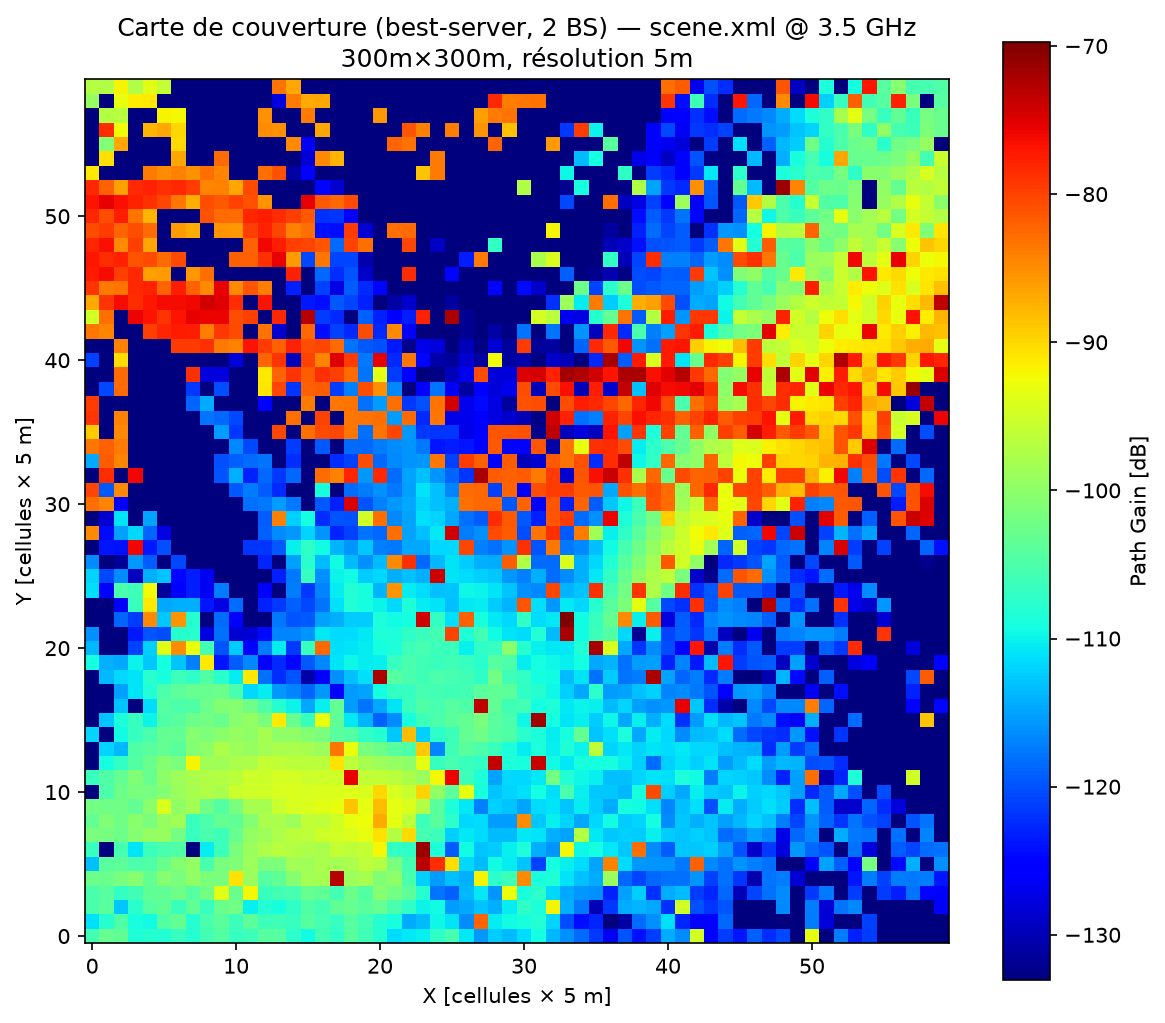
\includegraphics[width=0.75\textwidth]{radio_map_scene.png}
    \caption{Carte de couverture radio de la scène \texttt{scene.xml}.}
    \label{fig:radio_map}
\end{figure}

\begin{figure}[H]
    \centering
    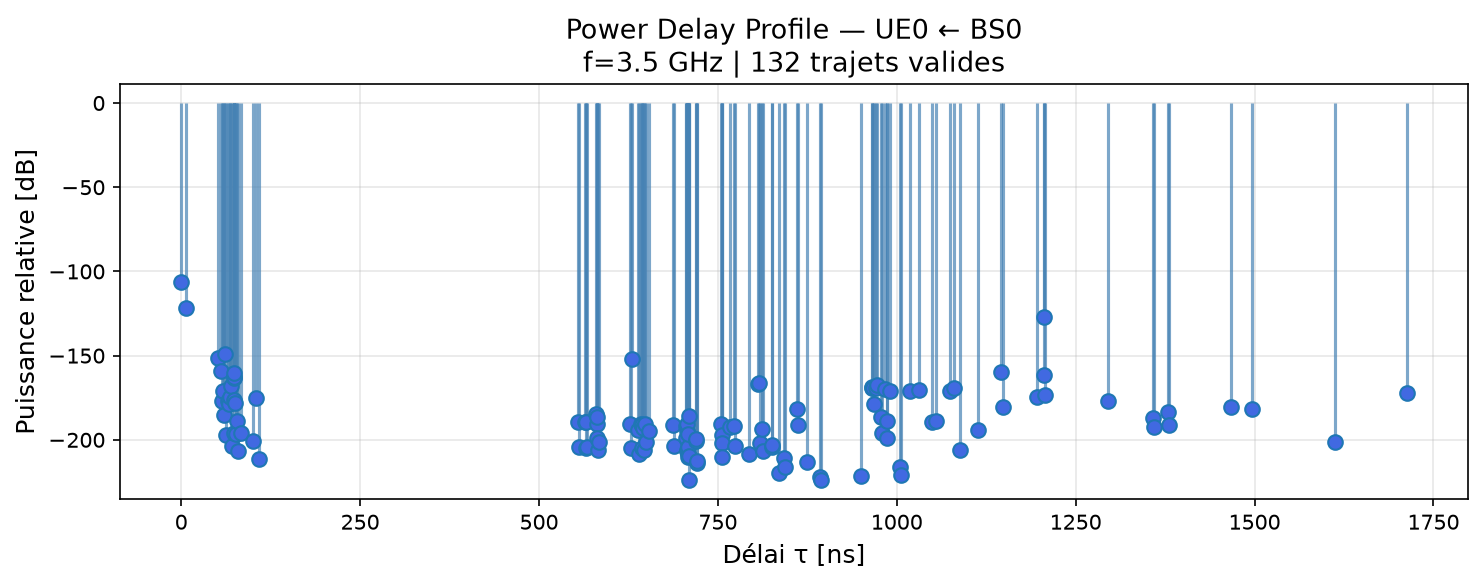
\includegraphics[width=0.48\textwidth]{pdp_ue0_bs0.png}
    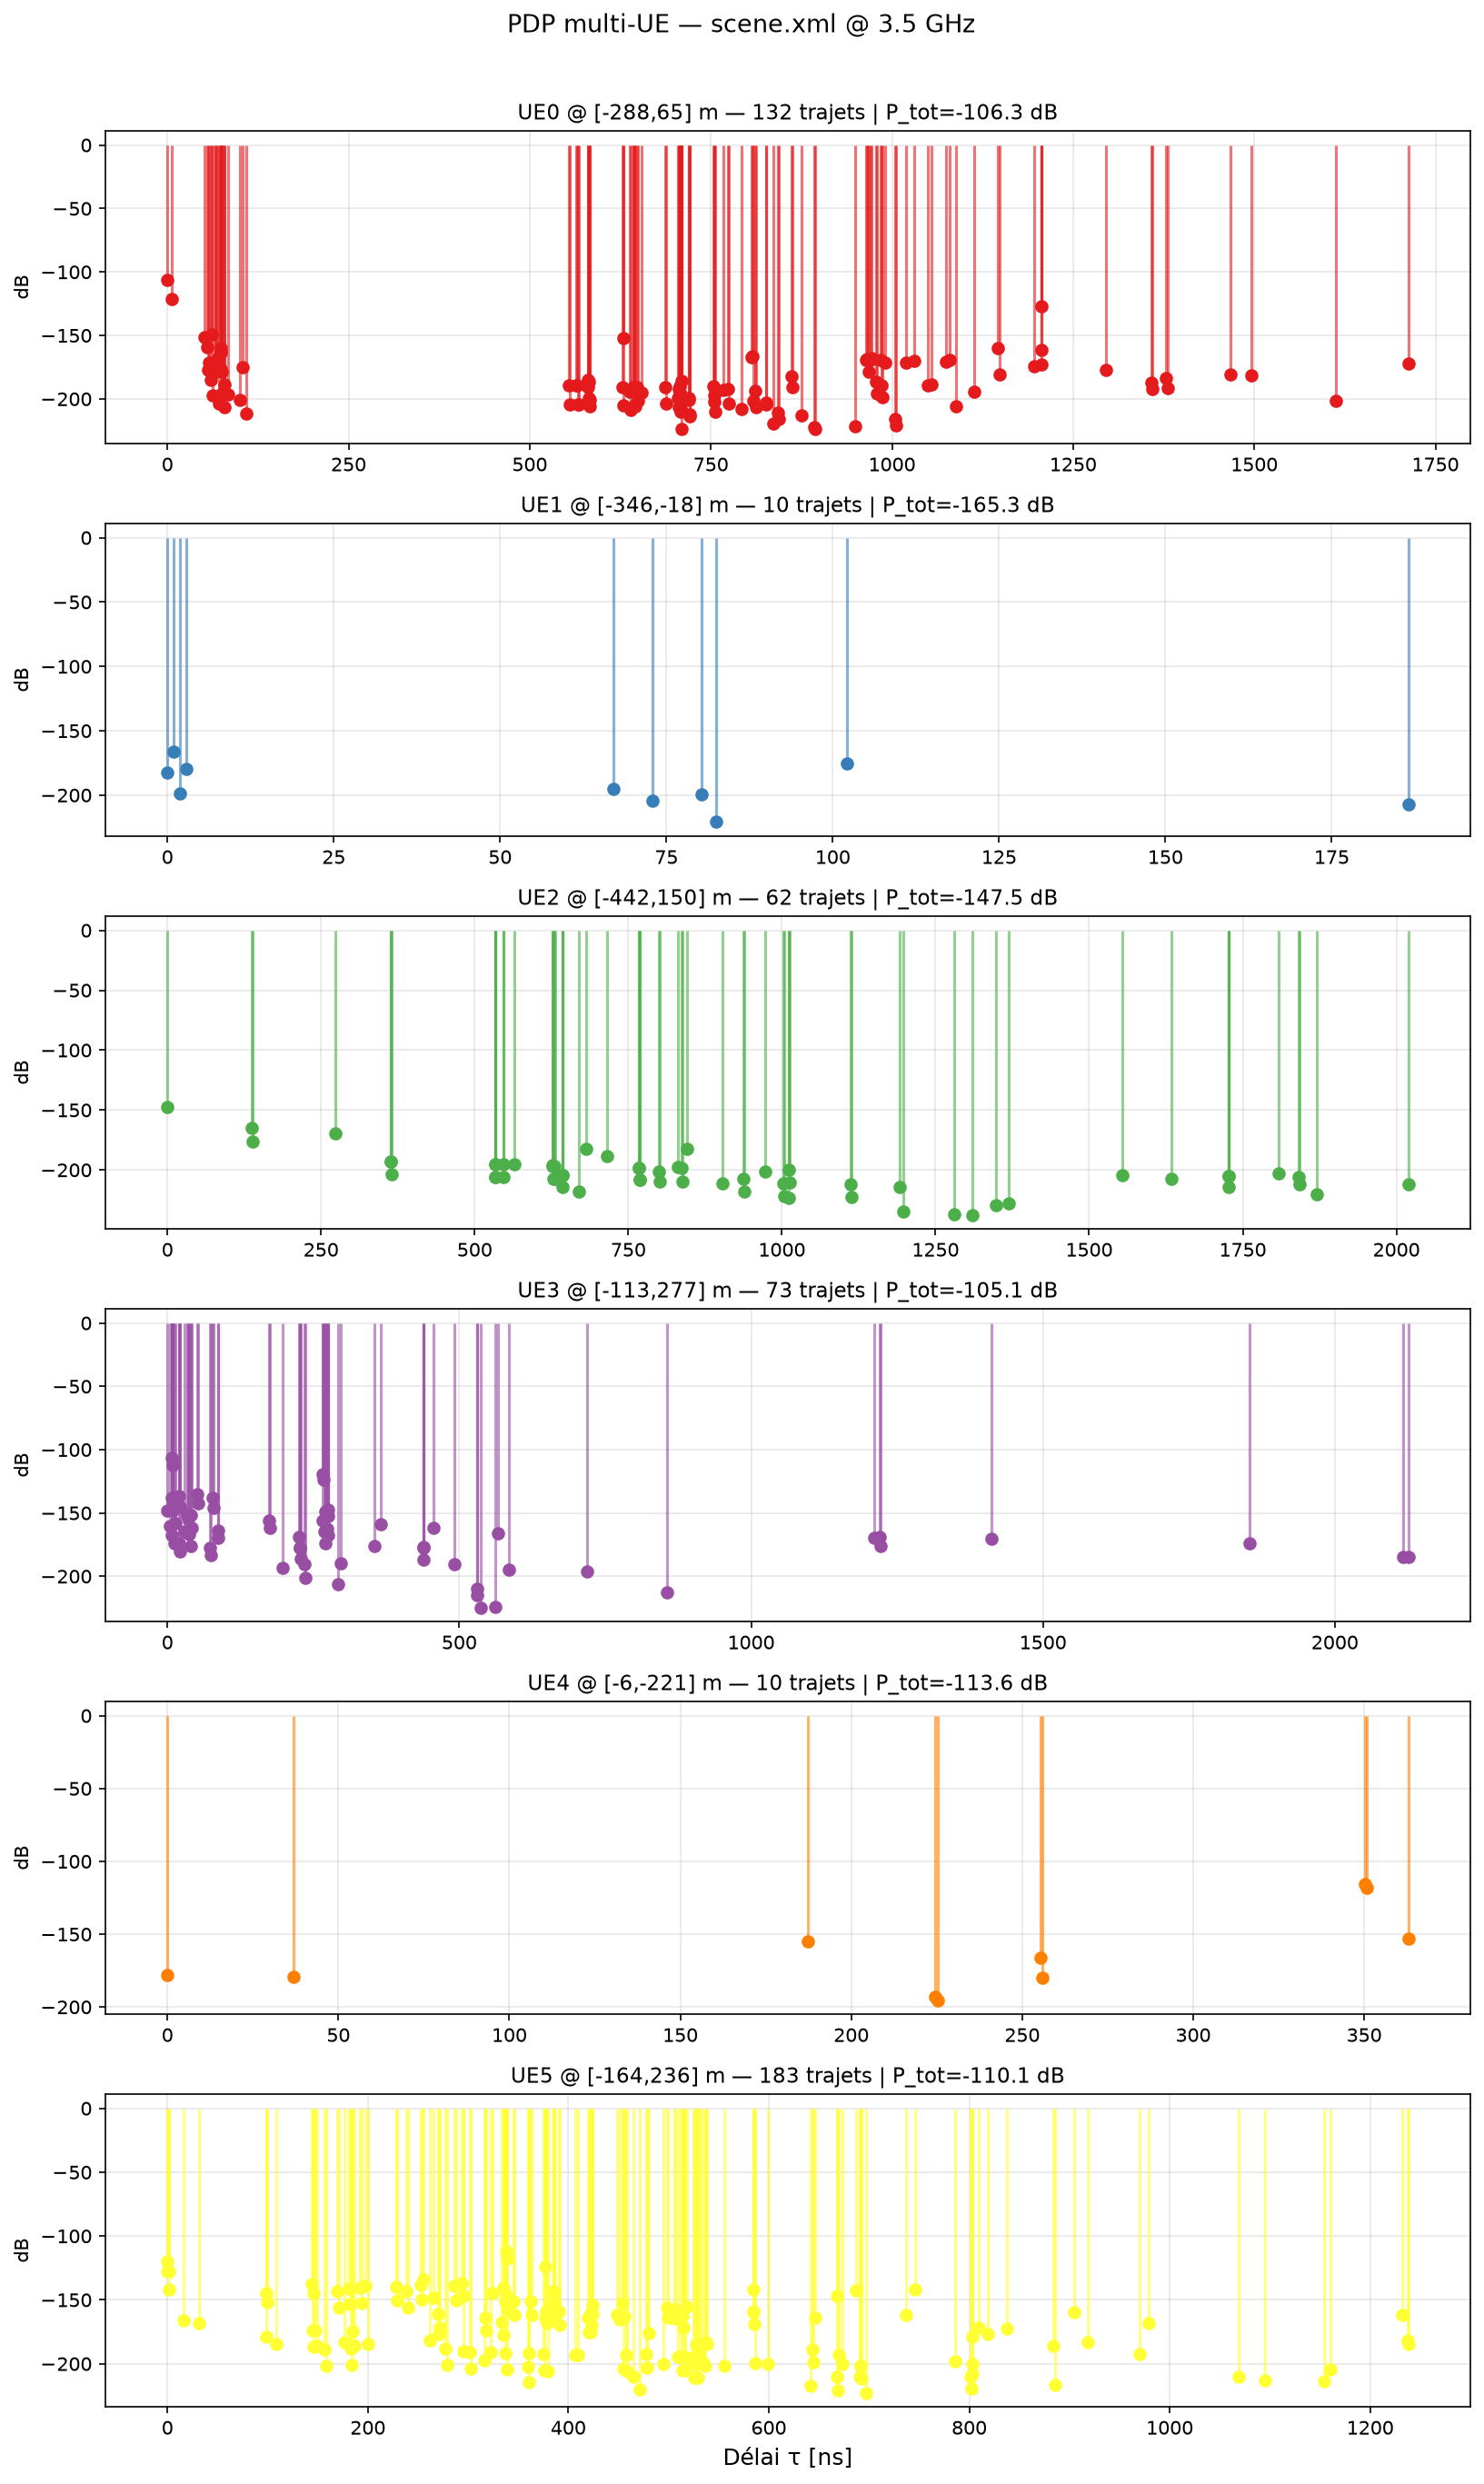
\includegraphics[width=0.48\textwidth]{pdp_all_ue.png}
    \caption{Profil de délai de puissance pour la liaison ue0--bs0 (gauche) et comparaison sur l'ensemble des UE (droite).}
    \label{fig:pdp}
\end{figure}

\subsection{Résultats de perception multimodale (modules 1b et 2)}
\label{subsec:res_phase3}

\begin{table}[H]
    \centering
    \caption{Résultats de fusion, architecture finale à 4 n\oe uds BS + 2 capteurs piétons.}
    \begin{tabular}{lc}
        \toprule
        \rowcolor{tabhead}
        \hd{Indicateur} & \hd{Valeur} \\
        \midrule
        Points radar totaux & 20\,899 \\
        \quad dont façade & 17\,425 \\
        \quad dont sol & 3\,119 \\
        \quad dont cible générique (\texttt{target}, avant fusion) & 355 \\
        Points fusionnés et raffinés en \texttt{car} & 315 \\
        Points fusionnés et raffinés en \texttt{pedestrian} & 37 \\
        Taux de raffinement des points \texttt{target} & $100\,\%$ (352/352) \\
        Contamination de points statiques par la vision & $0$ \\
        mAP50 (YOLOv8n fine-tuné) & $0{,}965$ \\
        mAP50-95 (YOLOv8n fine-tuné) & $0{,}887$ \\
        \bottomrule
    \end{tabular}
\end{table}

Le passage de l'architecture dual-n\oe ud (TX1/TX2) à l'architecture à quatre n\oe uds (ajout de TX3/TX4) a fait passer le nuage de points radar de 8\,038 à 20\,899 points et les objets fusionnés de 165 à 315 voitures et de 16 à 37 piétons --- une richesse multistatique nettement supérieure, illustrée en figure~\ref{fig:chart_growth}.

\begin{figure}[H]
    \centering
    \begin{tikzpicture}
    \begin{axis}[
        rapport,
        ybar, bar width=26pt,
        width=0.8\textwidth, height=6.5cm,
        symbolic x coords={Voitures fusionnées,Piétons fusionnés},
        xtick=data,
        ymin=0, ymax=370,
        ylabel={Objets fusionnés},
        legend style={at={(0.5,1.02)}, anchor=south, legend columns=-1},
        enlarge x limits=0.45,
        nodes near coords, nodes near coords style={font=\small},
    ]
    \addplot[altB] coordinates {(Voitures fusionnées,165)(Piétons fusionnés,16)};
    \addplot[choix] coordinates {(Voitures fusionnées,315)(Piétons fusionnés,37)};
    \legend{Architecture dual-n\oe ud (TX1/TX2), Architecture 4 n\oe uds (TX1--TX4)}
    \end{axis}
    \end{tikzpicture}
    \caption{Croissance des objets fusionnés lors du passage de l'architecture dual-n\oe ud à l'architecture à 4 n\oe uds.}
    \label{fig:chart_growth}
\end{figure}

\textbf{TX3} se comporte comme TX1/TX2 (détection vision confirmée). \textbf{TX4}, le n\oe ud le plus éloigné (180--210~m des acteurs), obtient \textbf{zéro détection vision} sur l'ensemble de la séquence : sa caméra est occultée par un bâtiment au premier plan, ce qu'a confirmé l'inspection visuelle de son rendu caméra. Sa contribution radar reste en revanche bien présente dans le nuage de points multistatique (Fig.~\ref{fig:radar_pointcloud}, 4\,678 points issus de TX4). Ce résultat est documenté comme une \textbf{limitation réaliste de déploiement} --- un site candidat n'offre pas toujours une ligne de vue dégagée sur toutes les cibles --- plutôt que corrigé artificiellement ; TX4 continue néanmoins d'apporter de la diversité radar multistatique.

\begin{figure}[H]
    \centering
    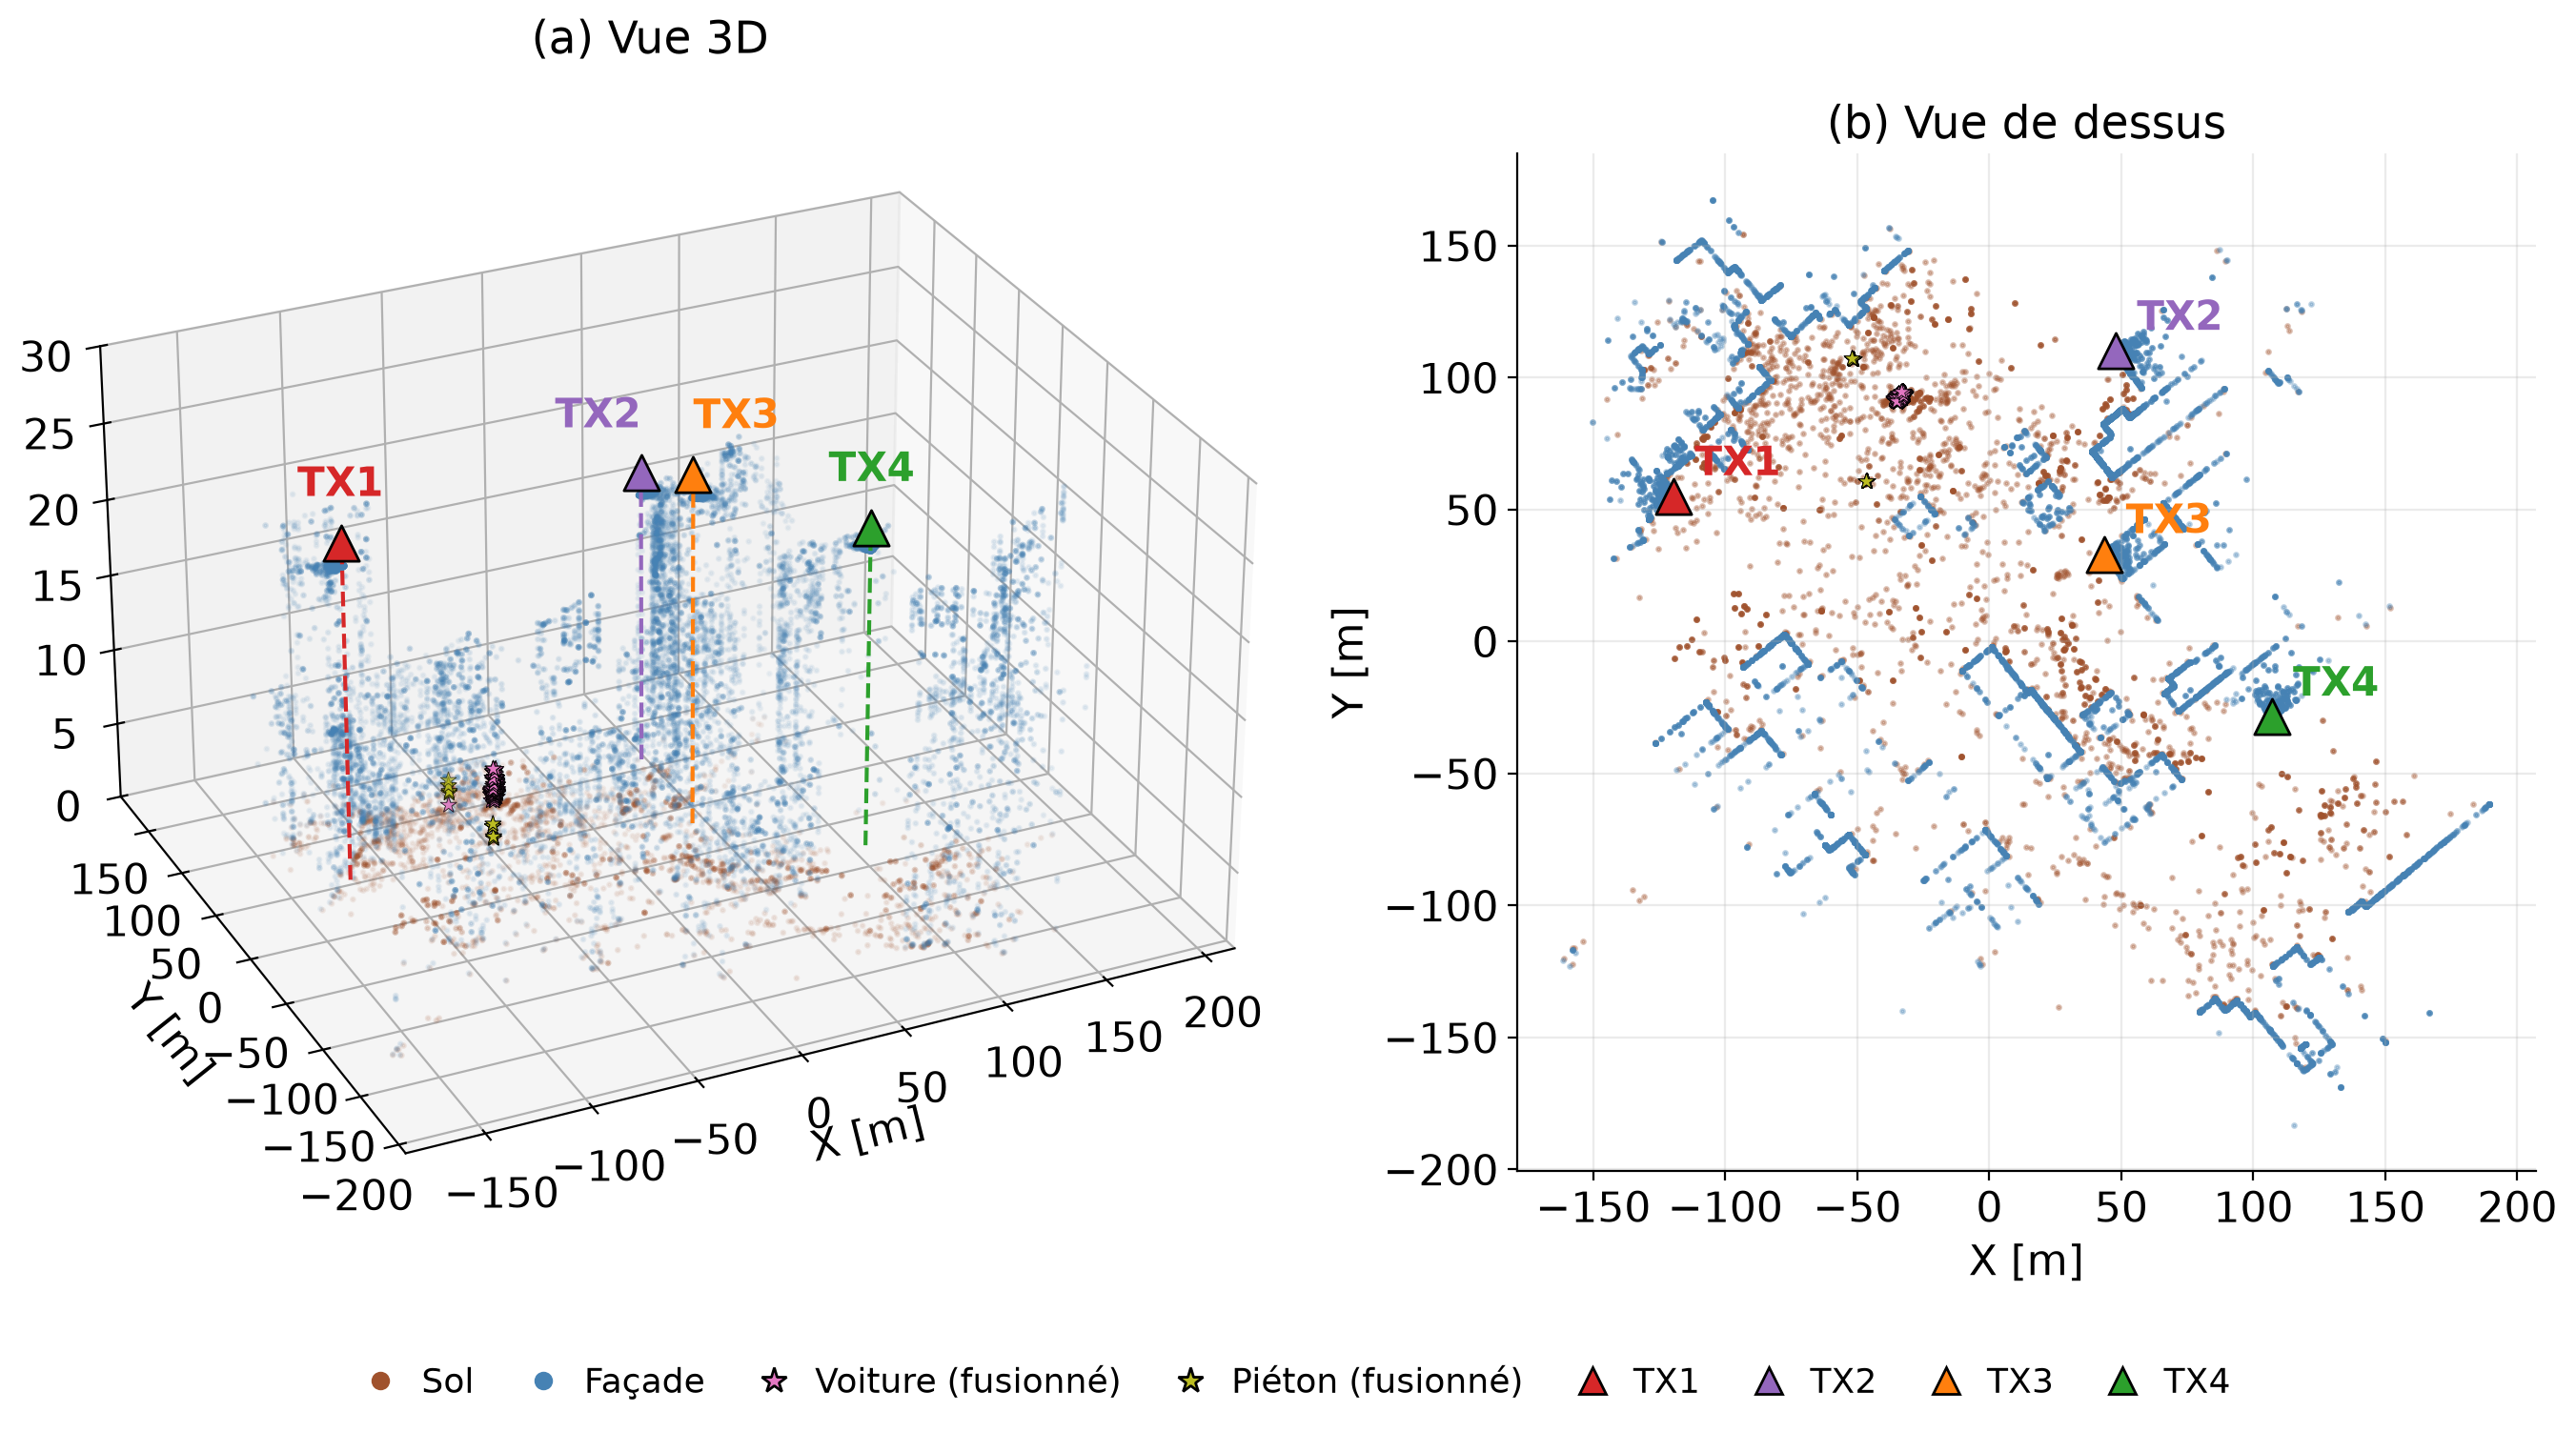
\includegraphics[width=\textwidth]{phase3/module1a_radar_pointcloud_v3.png}
    \caption{Nuage de points radar multistatique à 4 n\oe uds BS : (a) vue 3D, les pointillés matérialisant le mât de chaque n\oe ud ; (b) vue de dessus. Les points \texttt{target} y apparaissent sous leur classe raffinée après fusion (voiture, piéton).}
    \label{fig:radar_pointcloud}
\end{figure}

\subsubsection{Comportement sur la séquence dynamique (6 frames)}

La séquence dynamique (voiture à 1,5~m/frame, piétons à 0,8~m/frame, 6~frames) permet d'observer la stabilité du pipeline de fusion dans le temps. Le tableau~\ref{tab:res_dynamic} et la figure~\ref{fig:chart_dynamic} rapportent, frame par frame, le nombre de détections vision fusionnées par n\oe ud.

\begin{table}[H]
    \centering
    \caption{Détections vision fusionnées par n\oe ud, par frame (\texttt{phase3\_dynamic\_summary\_v2.json}).}
    \label{tab:res_dynamic}
    \begin{tabular}{lcccccc}
        \toprule
        \rowcolor{tabhead}
        \hd{Frame} & \hd{TX1} & \hd{TX2} & \hd{TX3} & \hd{TX4} & \hd{ped\_a} & \hd{ped\_b} \\
        \midrule
        0 & 1 & 1 & 1 & 0 & 2 & 2 \\
        1 & 1 & 2 & 1 & 0 & 2 & 2 \\
        2 & 1 & 3 & 1 & 0 & 2 & 2 \\
        3 & 1 & 4 & 2 & 0 & 2 & 2 \\
        4 & 3 & 3 & 2 & 0 & 2 & 2 \\
        5 & 3 & 3 & 3 & 0 & 2 & 2 \\
        \bottomrule
    \end{tabular}
\end{table}

\begin{figure}[H]
    \centering
    \begin{tikzpicture}
    \begin{axis}[
        rapport,
        width=0.9\textwidth, height=6.5cm,
        xlabel={Frame}, ylabel={Objets vision fusionnés},
        xtick={0,1,2,3,4,5},
        ymin=250, ymax=420,
        enlarge x limits=0.05,
        legend pos=south east,
        legend style={draw=gray!50, fill=white, fill opacity=0.9, text opacity=1},
    ]
    \addplot[color=cChoix, very thick, mark=*, mark options={fill=white, line width=1pt},
             nodes near coords, nodes near coords style={font=\small, color=cChoix, anchor=south, yshift=2pt}]
        coordinates {(0,353)(1,315)(2,331)(3,328)(4,322)(5,391)};
    \legend{Objets vision fusionnés (\texttt{vision\_matched})}
    \end{axis}
    \end{tikzpicture}
    \caption{Évolution du nombre d'objets vision fusionnés sur la séquence dynamique à 6 frames --- confirme que l'occultation de TX4 (0 détection, cf. Tableau~\ref{tab:res_dynamic}) persiste sur l'ensemble de la séquence, non un artefact d'une seule frame.}
    \label{fig:chart_dynamic}
\end{figure}

\subsection{Résultats de cartographie sémantique et encodage HD (module 3)}
\label{subsec:res_phase4}

La grille bayésienne 3D comporte $9 \times 169 \times 179 \times 6$ cellules (indexation Z, Y, X, classe), résolution 10~m en XY et 3~m en Z, soit $272\,259$ cellules spatiales dont $1\,449$ effectivement observées.

\begin{table}[H]
    \centering
    \caption{Résultats de l'encodage hyperdimensionnel.}
    \begin{tabular}{lc}
        \toprule
        \rowcolor{tabhead}
        \hd{Indicateur} & \hd{Valeur} \\
        \midrule
        Dimension de l'espace HD $D$ & $10\,000$ \\
        Niveaux par axe spatial & $64$ \\
        Ratio de compression (grille $\to$ vecteur HD) & $\times\,10\,454{,}7$ \\
        Classe retrouvée par similarité cosinus (requête position) & \texttt{car} ($0{,}379$) \\
        \bottomrule
    \end{tabular}
\end{table}

\begin{figure}[H]
    \centering
    \begin{tikzpicture}
    \begin{axis}[
        rapport,
        ybar, bar width=30pt, bar shift=0pt,
        width=0.8\textwidth, height=6.5cm,
        symbolic x coords={car,pedestrian,ground,facade},
        xtick={car,pedestrian,ground,facade},
        xticklabels={\textbf{car} (vérité terrain),pedestrian,ground,facade},
        ymin=0, ymax=0.45,
        ylabel={Similarité cosinus},
        enlarge x limits=0.18,
        nodes near coords, nodes near coords style={font=\small},
        /pgf/number format/.cd, use comma, fixed, zerofill, precision=3,
        /pgfplots/.cd, yticklabel style={/pgf/number format/.cd, zerofill=false, precision=1},
    ]
    \addplot[choix] coordinates {(car,0.379)};
    \addplot[altB] coordinates {(pedestrian,0.332)(ground,0.282)(facade,0.196)};
    \end{axis}
    \end{tikzpicture}
    \caption{Similarité cosinus par classe pour une requête position$\to$classe dont la vérité terrain est \texttt{car} --- la classe correcte obtient bien le score le plus élevé.}
    \label{fig:chart_hd_query}
\end{figure}

La requête position$\to$classe retrouve correctement la classe attendue (\texttt{car}) avec la similarité la plus élevée, validant le mécanisme d'encodage (équation~\eqref{eq:hd_encoding}) après correction de deux pièges de capacité HDC : (i) un calage initial des niveaux sur la boîte englobante complète de la scène ($\sim$1800~m) écrasait le signal utile, résolu en calant la plage sur l'étendue \textbf{réellement observée} ($\sim$250~m) ; (ii) un \textit{bundle} plat laissait une classe nombreuse (façade, $\sim$800 cellules) noyer une classe rare (voiture, 1--3 cellules), résolu en bundlant les positions \textbf{par classe d'abord} (cf. listing de \S\ref{sec:methodologie}).

\begin{table}[H]
    \centering
    \caption{Fusion multi-BS par addition de vecteurs HD --- similarité à la carte complète.}
    \begin{tabular}{lc}
        \toprule
        \rowcolor{tabhead}
        \hd{Configuration} & \hd{Similarité cosinus} \\
        \midrule
        bs2 (TX3) seul (meilleur n\oe ud individuel) & $0{,}752$ \\
        bs0 seul & $0{,}689$ \\
        bs1 seul & $0{,}668$ \\
        bs3 (TX4) seul & $0{,}520$ \\
        Fusion par addition simple (4 n\oe uds) & $0{,}617$ \\
        Fusion pondérée par confiance caméra (4 n\oe uds) & $0{,}597$ \\
        \bottomrule
    \end{tabular}
\end{table}

\begin{figure}[H]
    \centering
    \begin{tikzpicture}
    \begin{axis}[
        rapport,
        ybar, bar width=24pt, bar shift=0pt,
        width=\textwidth, height=6.8cm,
        symbolic x coords={bs0,bs1,bs2,bs3,Fsimple,Fpond},
        xtick={bs0,bs1,bs2,bs3,Fsimple,Fpond},
        xticklabels={bs0 (TX1),bs1 (TX2),bs2 (TX3),bs3 (TX4),Fusion simple,Fusion pondérée},
        x tick label style={font=\small, align=center, text width=1.8cm},
        ymin=0, ymax=0.85,
        ylabel={Similarité cosinus à la carte complète},
        enlarge x limits=0.1,
        nodes near coords, nodes near coords style={font=\small},
        /pgf/number format/.cd, use comma, fixed, zerofill, precision=3,
        /pgfplots/.cd, yticklabel style={/pgf/number format/.cd, zerofill=false, precision=1},
        legend style={at={(0.5,1.02)}, anchor=south, legend columns=-1},
    ]
    \addplot[fill=cChoix!45, draw=cChoix, area legend] coordinates {(bs0,0.689)(bs1,0.668)(bs3,0.520)};
    \addplot[choix] coordinates {(bs2,0.752)};
    \addplot[altA] coordinates {(Fsimple,0.617)(Fpond,0.597)};
    \draw[dashed, thick, cChoix] ({rel axis cs:0,0}|-{axis cs:bs0,0.752}) -- ({rel axis cs:1,0}|-{axis cs:bs0,0.752})
        node[pos=0.98, above, font=\scriptsize, anchor=south east] {meilleur n\oe ud individuel};
    \legend{N\oe ud individuel, Meilleur n\oe ud (bs2), Fusion HD (4 n\oe uds)}
    \end{axis}
    \end{tikzpicture}
    \caption{Similarité cosinus par n\oe ud individuel vs. fusion multi-BS par addition HD --- le meilleur n\oe ud individuel (bs2) dépasse les deux variantes de fusion au-delà de 2--3 n\oe uds.}
    \label{fig:chart_hd_fusion}
\end{figure}

Avec deux n\oe uds (bs0+bs1), la fusion par addition de vecteurs HD dépassait chaque n\oe ud pris isolément, validant le principe de fusion multi-BS envisagé (\S\ref{subsec:pipeline_six_modules}). \textbf{Ce résultat ne se maintient plus à quatre n\oe uds} : la fusion (pondérée ou non) reste en dessous du meilleur n\oe ud individuel (bs2, $0{,}752$), comme le montre la figure~\ref{fig:chart_hd_fusion}. Diagnostic : chaque vecteur par n\oe ud est déjà seuillé en bipolaire avant sommation (contrainte de compression backhaul), et avec seulement 3--4 vecteurs à sommer, les égalités de vote majoritaire deviennent fréquentes --- une \textbf{limitation de capacité intrinsèque au bundling bipolaire HDC}, non un défaut d'implémentation. Ce constat est documenté explicitement (notebook et \texttt{phase4\_summary.json}) et \textbf{circonscrit à cette démonstration de compression} : la grille bayésienne 3D elle-même, qui constitue le jumeau numérique de référence, intègre correctement les six n\oe uds par mise à jour bayésienne directe, sans passer par ce seuillage bipolaire intermédiaire.

\begin{figure}[H]
    \centering
    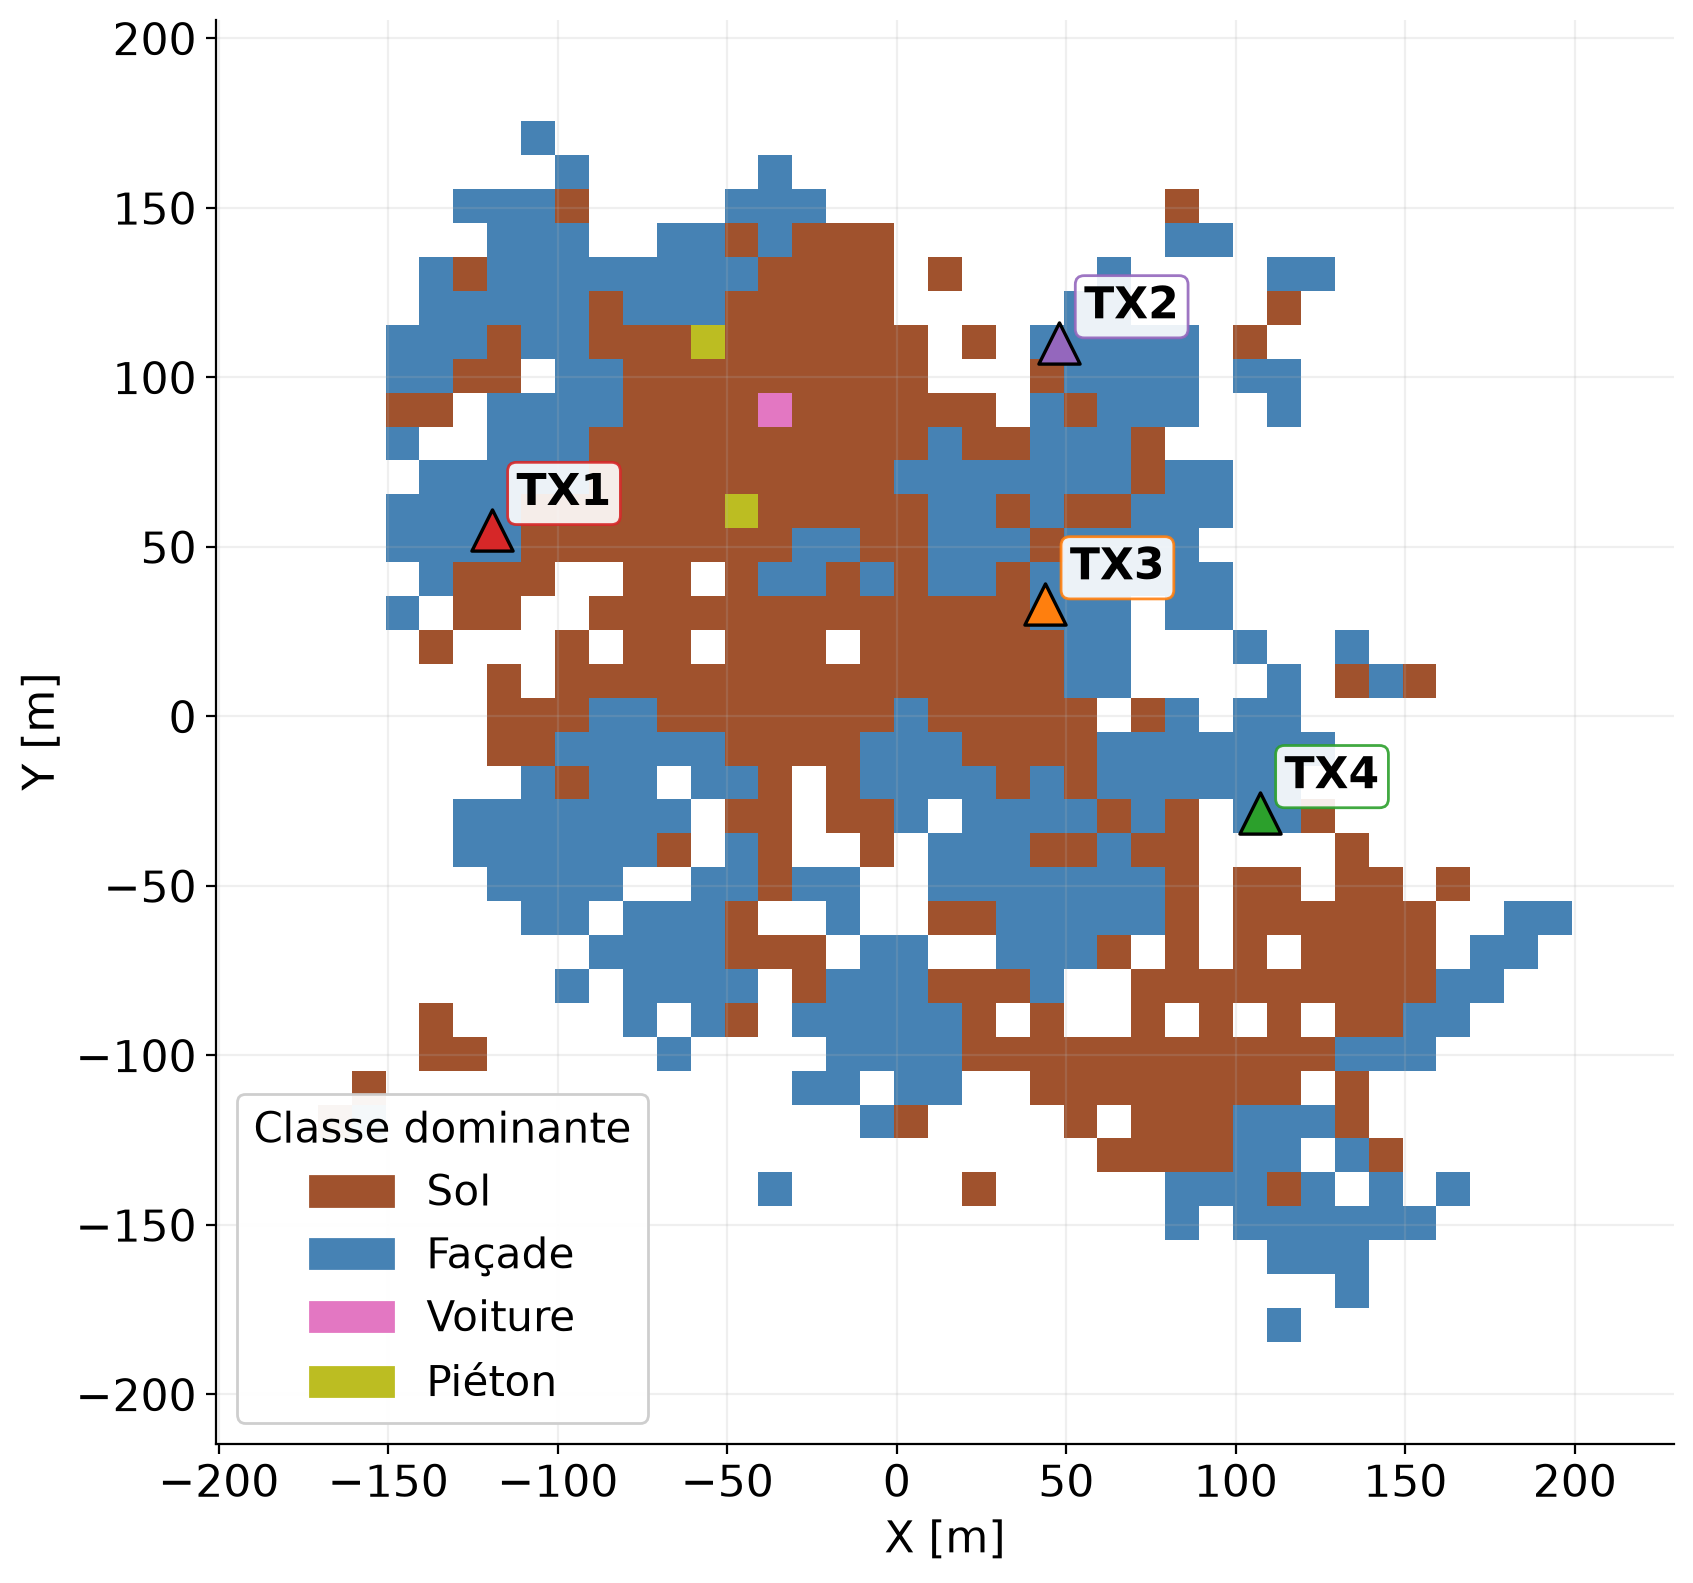
\includegraphics[width=0.82\textwidth]{phase4/module3_grid3d_topdown_v3.png}
    \caption{Projection top-down de la grille bayésienne 3D (classe dominante par colonne, cellules de 10~m), recadrée sur la zone observée.}
    \label{fig:phase4_topdown}
\end{figure}

\begin{figure}[H]
    \centering
    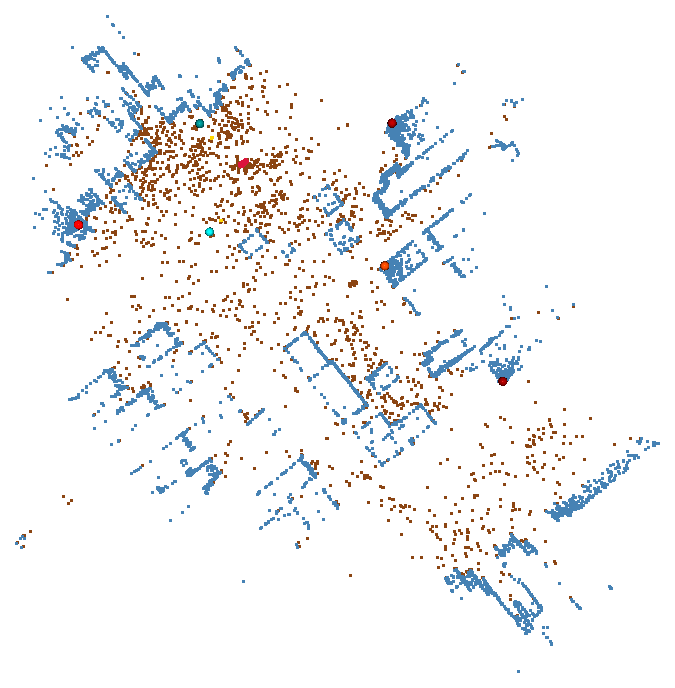
\includegraphics[width=0.82\textwidth]{phase4/module3_open3d_pointcloud_cropped.png}
    \caption{Rendu Open3D du nuage de points sémantique coloré par classe, avec les 6 n\oe uds de sensing.}
    \label{fig:phase4_open3d}
\end{figure}

\subsection{Synthèse des résultats}

\begin{table}[H]
    \centering
    \caption{Synthèse des résultats obtenus.}
    \begin{tabularx}{\textwidth}{F{3.8cm}L}
        \toprule
        \rowcolor{tabhead}
        \hd{Module} & \hd{Résultat principal} \\
        \midrule
        1a. Acquisition ISAC & Environnement Sionna RT fonctionnel, 6 liaisons BS--UE simulées, validation complète (scène, trajets, CIR, PDP) \\
        1b + 2. Acquisition vision et fusion & 20\,899 points radar multistatiques, 315 voitures + 37 piétons correctement fusionnés (100\,\% des points \texttt{target}, 0 contamination), détecteur YOLOv8n mAP50~$=0{,}965$, comportement stable sur 6 frames dynamiques \\
        3. Cartographie sémantique & Grille bayésienne 3D (1\,449 cellules observées), encodage HD validé (requête correcte, compression $\times10\,454$), limitation de capacité HDC en fusion multi-BS documentée au-delà de 2--3 n\oe uds \\
        \bottomrule
    \end{tabularx}
\end{table}

% ============================================================
\section{Limitations et Périmètre du Projet}
\label{sec:limitations}
% ============================================================

Conformément à une démarche d'ingénierie honnête, les écarts suivants par rapport à l'architecture visée (\S\ref{sec:architecture_proposee}) sont documentés et justifiés plutôt que masqués.

\begin{itemize}[leftmargin=1.5em]
    \item \textbf{Fréquence porteuse} : le cahier des charges visait la bande mmWave (28~GHz) ; le pipeline fonctionne à 3,5~GHz. Cause : le matériau de sol \texttt{itu\_very\_dry\_ground} n'est défini par l'ITU-R P.2040 que pour la plage 1--10~GHz. Passer à 28~GHz nécessite d'abord de substituer ce matériau par \texttt{itu\_concrete} (valide 1--100~GHz).
    \item \textbf{Hauteur des stations de base} : visée à 10~m, les quatre n\oe uds sont en réalité montés en toiture ($\sim$18--23~m), choisis pour garantir une ligne de vue directe sur les acteurs. Il s'agit d'un déploiement rooftop réaliste, à assumer plutôt qu'à corriger.
    \item \textbf{TX4 sans confirmation vision} : occultation par un bâtiment au premier plan (\S\ref{subsec:res_phase3}) --- limitation de déploiement réaliste, non une erreur de conception.
    \item \textbf{Fusion multi-BS par addition HD} : ne dépasse plus le meilleur n\oe ud individuel au-delà de 2--3 n\oe uds (\S\ref{subsec:res_phase4}) --- limitation de capacité du bundling bipolaire, circonscrite à cette démonstration de compression.
    \item \textbf{Suivi temporel} : l'association radar-vision est indépendante par frame (\S\ref{subsec:art_tracking}) ; un filtre de suivi complet (Kalman/JPDA) n'a pas été implémenté, la séquence testée (6 frames) restant courte.
    \item \textbf{SegFormer non utilisé} : le module 1b (\S\ref{subsec:pipeline_six_modules}) proposait YOLOv8-seg \textit{ou} SegFormer ; seul YOLOv8 a été mis en \oe uvre (\S\ref{sec:choix_tech}).
    \item \textbf{Modules 4 à 6 de l'architecture} (carte de risque, JSCC, apprentissage fédéré, interface \textit{World Model} AGI, \S\ref{subsec:pipeline_six_modules}) : leurs interfaces sont spécifiées dans l'architecture proposée mais leur implémentation constitue une direction d'exploitation distincte de la carte sémantique, volontairement hors du périmètre retenu pour ce rapport, qui porte sur la construction et la validation de la carte elle-même (modules 1a, 1b, 2, 3).
\end{itemize}

% ============================================================
\section{Conclusion Générale}
\label{sec:conclusion}
% ============================================================

Ce rapport a présenté, de la revue de littérature à la validation expérimentale, le projet SDM-VA-ISAC : positionné par rapport aux architectures fondatrices AGI-native (\textit{Telecom Brain}) et SA-VA-ISAC (\S\ref{sec:etat_art}), l'architecture globale proposée en six modules (\S\ref{sec:architecture_proposee}) répond à la lacune identifiée --- l'absence de spécification concrète du pont entre signaux physiques et représentation sémantique --- par un pipeline de perception et de cartographie complet et validé sur son périmètre d'implémentation (modules 1a, 1b, 2, 3) : un environnement de simulation Sionna RT calibré sur une scène urbaine réelle, un pipeline de perception multimodale à six n\oe uds de sensing associant ISAC et vision fine-tunée par fusion KD-tree, et une carte sémantique 3D compressée par encodage hyperdimensionnel avec visualisation interactive.

Chaque choix technologique structurant a été comparé explicitement --- tableaux et graphiques à l'appui --- à ses alternatives et justifié par l'expérience d'implémentation (\S\ref{sec:choix_tech}), et chaque limitation rencontrée --- occultation de TX4, capacité de fusion HD au-delà de 2--3 n\oe uds, écarts de fréquence et de hauteur d'antenne, absence de suivi temporel complet --- a été diagnostiquée et documentée plutôt que masquée (\S\ref{sec:limitations}).

La carte sémantique 3D validée, en particulier sa forme compressée par encodage hyperdimensionnel, constitue le pont opérationnel entre couche physique et représentation sémantique identifié comme lacune dans la revue de littérature --- une brique directement réutilisable pour l'exploitation applicative envisagée par les modules 4 à 6 de l'architecture proposée (carte de risque sémantique, compression JSCC, interface avec un modèle du monde causal), sans que leur réalisation soit nécessaire pour clore le présent périmètre.

\newpage
% ============================================================
%  RÉFÉRENCES
% ============================================================
\begin{thebibliography}{99}

\bibitem{saad2025}
W. Saad \textit{et al.},
``Artificial General Intelligence (AGI)-Native Wireless Systems: A Journey Beyond 6G,''
\textit{arXiv preprint}, 2025.

\bibitem{sa_va_isac_main}
Auteur(s) de l'article source,
``Semantic-Aware Vision-Assisted ISAC Architecture and Resource Allocation,''
\textit{IEEE Journal}, 2024.

\bibitem{shannon1948}
C. E. Shannon,
``A Mathematical Theory of Communication,''
\textit{Bell System Technical Journal}, vol.~27, pp.~379--423, 1948.

\bibitem{pearl2009}
J. Pearl,
\textit{Causality: Models, Reasoning and Inference}, 2nd ed.
Cambridge University Press, 2009.

\bibitem{isac_survey}
F.~Liu \textit{et al.},
``Integrated Sensing and Communications: Toward Dual-Functional Wireless Networks for 6G and Beyond,''
\textit{IEEE JSAC}, vol.~40, no.~6, pp.~1728--1767, 2022.

\bibitem{semantic_comm}
H.~Xie \textit{et al.},
``Deep Learning Enabled Semantic Communication Systems,''
\textit{IEEE Trans. Signal Process.}, vol.~69, pp.~2663--2675, 2021.

\bibitem{drl_beamforming}
W.~Cui, K.~Shen, W.~Yu,
``Spatial Deep Learning for Wireless Scheduling,''
\textit{IEEE JSAC}, vol.~37, no.~6, pp.~1248--1261, 2019.

\bibitem{vision_isac}
Y. Gao \textit{et al.},
``Vision-Aided ISAC in Low-Altitude Economy Networks via De-Diffused Visual Priors,''
\textit{arXiv:2507.01574}, 2025.

\bibitem{cell_free_mimo}
Ö.~T.~Demir, E.~Björnson, L.~Sanguinetti,
``Foundations of User-Centric Cell-Free Massive MIMO,''
\textit{Found. Trends Signal Process.}, vol.~14, no.~3--4, pp.~162--472, 2021.

\bibitem{federated_learning}
H.~B.~McMahan \textit{et al.},
``Communication-Efficient Learning of Deep Networks from Decentralized Data,''
in \textit{Proc. AISTATS}, 2017, pp.~1273--1282.

\bibitem{sionna_rt_2}
J. Hoydis \textit{et al.},
``Sionna RT: Differentiable Ray Tracing for Radio Propagation Modeling,''
\textit{arXiv:2303.11103}, 2023.

\bibitem{sionna}
J. Hoydis \textit{et al.},
``Sionna: An Open-Source Library for Next-Generation Physical Layer Research,''
\textit{arXiv:2203.11854}, 2022.

\bibitem{remcom_wi}
Remcom Inc.,
``Wireless InSite Propagation Software --- User's Manual,'' 2023.

\bibitem{ultralytics_yolov8}
G. Jocher, A. Chaurasia, J. Qiu,
``Ultralytics YOLOv8,''
\url{https://github.com/ultralytics/ultralytics}, 2023.

\bibitem{segformer}
E. Xie, W. Wang, Z. Yu, A. Anandkumar, J. M. Alvarez, P. Luo,
``SegFormer: Simple and Efficient Design for Semantic Segmentation with Transformers,''
in \textit{Proc. NeurIPS}, 2021.

\bibitem{domain_randomization}
J. Tobin, R. Fong, A. Ray, J. Schneider, W. Zaremba, P. Abbeel,
``Domain Randomization for Transferring Deep Neural Networks from Simulation to the Real World,''
in \textit{Proc. IROS}, 2017.

\bibitem{bar_shalom_tracking}
Y. Bar-Shalom, T. E. Fortmann,
``Tracking and Data Association,''
Academic Press, 1988.

\bibitem{bentley_kdtree}
J. L. Bentley,
``Multidimensional Binary Search Trees Used for Associative Searching,''
\textit{Communications of the ACM}, vol.~18, no.~9, pp.~509--517, 1975.

\bibitem{elfes_occupancy}
A. Elfes,
``Using Occupancy Grids for Mobile Robot Perception and Navigation,''
\textit{IEEE Computer}, vol.~22, no.~6, pp.~46--57, 1989.

\bibitem{thrun_occupancy}
S. Thrun,
``Learning Occupancy Grid Maps with Forward Sensor Models,''
\textit{Autonomous Robots}, vol.~15, pp.~111--127, 2003.

\bibitem{grieves_digital_twin}
M. Grieves, J. Vickers,
``Digital Twin: Mitigating Unpredictable, Undesirable Emergent Behavior in Complex Systems,''
in \textit{Transdisciplinary Perspectives on Complex Systems}, Springer, 2017.

\bibitem{kanerva_hdc}
P. Kanerva,
``Hyperdimensional Computing: An Introduction to Computing in Distributed Representation with High-Dimensional Random Vectors,''
\textit{Cognitive Computation}, vol.~1, pp.~139--159, 2009.

\bibitem{plate_hrr}
T. A. Plate,
``Holographic Reduced Representations,''
\textit{IEEE Trans. Neural Networks}, vol.~6, no.~3, pp.~623--641, 1995.

\bibitem{rahimi_hdc}
A. Rahimi, P. Kanerva, J. M. Rabaey,
``A Robust and Energy-Efficient Classifier Using Brain-Inspired Hyperdimensional Computing,''
in \textit{Proc. ISLPED}, 2016.

\bibitem{open3d}
Q.-Y. Zhou, J. Park, V. Koltun,
``Open3D: A Modern Library for 3D Data Processing,''
\textit{arXiv:1801.09847}, 2018.

\end{thebibliography}

\end{document}
